%% BioMed_Central_Tex_Template_v1.06
%%                                      %
%  bmc_article.tex            ver: 1.06 %
%                                       %

%%IMPORTANT: do not delete the first line of this template
%%It must be present to enable the BMC Submission system to
%%recognise this template!!

%%%%%%%%%%%%%%%%%%%%%%%%%%%%%%%%%%%%%%%%%
%%                                     %%
%%  LaTeX template for BioMed Central  %%
%%     journal article submissions     %%
%%                                     %%
%%          <8 June 2012>              %%
%%                                     %%
%%                                     %%
%%%%%%%%%%%%%%%%%%%%%%%%%%%%%%%%%%%%%%%%%


%%%%%%%%%%%%%%%%%%%%%%%%%%%%%%%%%%%%%%%%%%%%%%%%%%%%%%%%%%%%%%%%%%%%%
%%                                                                 %%
%% For instructions on how to fill out this Tex template           %%
%% document please refer to Readme.html and the instructions for   %%
%% authors page on the biomed central website                      %%
%% http://www.biomedcentral.com/info/authors/                      %%
%%                                                                 %%
%% Please do not use \input{...} to include other tex files.       %%
%% Submit your LaTeX manuscript as one .tex document.              %%
%%                                                                 %%
%% All additional figures and files should be attached             %%
%% separately and not embedded in the \TeX\ document itself.       %%
%%                                                                 %%
%% BioMed Central currently use the MikTex distribution of         %%
%% TeX for Windows) of TeX and LaTeX.  This is available from      %%
%% http://www.miktex.org                                           %%
%%                                                                 %%
%%%%%%%%%%%%%%%%%%%%%%%%%%%%%%%%%%%%%%%%%%%%%%%%%%%%%%%%%%%%%%%%%%%%%

\documentclass[doublespacing,linenumbers]{bmcart}
%\documentclass[doublespacing,linenumbers]{bmcart-modified}
%% bmcart-modified increases the spacing between the line numbers and the text.


%%% Load packages
\usepackage[utf8]{inputenc} 
\usepackage{graphicx}
\usepackage{amssymb,amsfonts,amsmath,bm,xspace} %bm provides a complete and easy to use set of bold math fonts using \bm{}
\usepackage{dsfont} %provides \mathds{G}
\usepackage{paralist}
%\usepackage{ifthen}
\usepackage{url}
%\usepackage{caption}
%\usepackage{titling} %provides \theauthor and \thetitle commands
\usepackage{natbib}
\usepackage{color}
%\usepackage{multirow}
\usepackage{subfigure}

\usepackage[flushleft]{threeparttable}

%%%%%%%%%%%%%%%%%%%%%%%%%%%%%%%%%%%%%%%%%%%%%%%%%
%%                                             %%
%%  If you wish to display your graphics for   %%
%%  your own use using includegraphic or       %%
%%  includegraphics, then comment out the      %%
%%  following two lines of code.               %%
%%  NB: These line *must* be included when     %%
%%  submitting to BMC.                         %%
%%  All figure files must be submitted as      %%
%%  separate graphics through the BMC          %%
%%  submission process, not included in the    %%
%%  submitted article.                         %%
%%                                             %%
%%%%%%%%%%%%%%%%%%%%%%%%%%%%%%%%%%%%%%%%%%%%%%%%%

\def\includegraphic{}
\def\includegraphics{}


%%% Put your definitions there:
\startlocaldefs

%% Remove line numbers from left side
%% see: https://tex.stackexchange.com/a/227374
%\usepackage{etoolbox}
%\makeatletter
%\patchcmd\set@numberlines@box{\rlap}{\@gobble}{}{}
%\makeatother


\newcommand\suppl{\par
  \setcounter{section}{0}%
  \setcounter{subsection}{0}%
  \setcounter{table}{0}%
  \setcounter{figure}{0}%
  \setcounter{equation}{0}%
  \gdef\thesection{\Alph{section}.1}%
  \def\thefigure{\Alph{section}\arabic{figure}}%
  \def\thetable{\Alph{section}\arabic{table}}%
  \def\theequation {\Alph{section}\arabic{equation}}}


  \newcommand{\package}{\textbf{AnaCoDa}\xspace} % Use xspace, not two commands!
  \newcommand{\kluyveri}{\textit{L. kluyveri}\xspace}
  \newcommand{\dubl}{\textit{C. dubliniensis}\xspace}
  \newcommand{\gossypii}{\textit{E. gossypii}\xspace}
  \newcommand{\ROC}{ROC SEMPPR\xspace}
  \newcommand{\GC}{GC content\xspace}
  \newcommand{\DM}{\ensuremath{{\Delta M}}\xspace}
  \newcommand{\DE}{\ensuremath{{\Delta \eta}}\xspace}
  \newcommand{\Ne}{\ensuremath{N_e}\xspace}
  \newcommand{\Lik}{\ensuremath{\mathcal{L}}\xspace}
  \newcommand{\GL}{\ensuremath{{\Delta s}}\xspace}
  
\endlocaldefs

\begin{document}
  
%%% Start of article front matter
\begin{frontmatter}

\begin{fmbox}
\dochead{Research}  
  
 %%%%%%%%%%%%%%%%%%%%%%%%%%%%%%%%%%%%%%%%%%%%%%
%%                                          %%
%% Enter the title of your article here     %%
%%                                          %%
%%%%%%%%%%%%%%%%%%%%%%%%%%%%%%%%%%%%%%%%%%%%%%
\title{Unlocking a signal of introgression from codons in Lachancea kluveri using a mutation-selection model}

%%%%%%%%%%%%%%%%%%%%%%%%%%%%%%%%%%%%%%%%%%%%%%
%%                                          %%
%% Enter the authors here                   %%
%%                                          %%
%% Specify information, if available,       %%
%% in the form:                             %%
%%   <key>={<id1>,<id2>}                    %%
%%   <key>=                                 %%
%% Comment or delete the keys which are     %%
%% not used. Repeat \author command as much %%
%% as required.                             %%
%%                                          %%
%%%%%%%%%%%%%%%%%%%%%%%%%%%%%%%%%%%%%%%%%%%%%%
\author[
   addressref={aff1, aff2, aff3},                   % id's of addresses, e.g. {aff1,aff2}
   corref={aff3},                       % id of corresponding address, if any
   %noteref={n1},                        % id's of article notes, if any
   email={cedric.landerer@gmail.com}   % email address
]{\inits{C}\fnm{Cedric} \snm{Landerer}}
\author[
   addressref={aff1,aff2},
   email={bomeara@utk.edu}
]{\inits{BC}\fnm{Brian C} \snm{O'Meara}}
\author[
   addressref={aff2,aff4},
   email={russell.zaretzki@gmail.com}
]{\inits{R}\fnm{Russell} \snm{Zaretzki}}
\author[
   addressref={aff1,aff2},
   email={mikeg@utk.edu}
]{\inits{MA}\fnm{Michael A} \snm{Gilchrist}}

%%%%%%%%%%%%%%%%%%%%%%%%%%%%%%%%%%%%%%%%%%%%%%
%%                                          %%
%% Enter the authors' addresses here        %%
%%                                          %%
%% Repeat \address commands as much as      %%
%% required.                                %%
%%                                          %%
%%%%%%%%%%%%%%%%%%%%%%%%%%%%%%%%%%%%%%%%%%%%%%

\address[id=aff1]{%                           % unique id
  \orgname{Department of Ecology \& Evolutionary  Biology, University of Tennessee}, % university, etc
  %\street{Waterloo Road},                     %
  \postcode{37996},                           % post or zip code
  \city{Knoxville, TN},                              % city
  \cny{USA}                                    % country
}
\address[id=aff2]{%
  \orgname{National Institute for Mathematical and Biological Synthesis},
  \postcode{37996},
  \city{Knoxville, TN},
  \cny{USA}
}
\address[id=aff3]{%
  \orgname{Max-Planck Institute of Molecular Cell Biology and Genetics},
  \street{Pfotenhauerstr. 108},
  \postcode{01307},
  \city{Dresden},
  \cny{Germany}
}
\address[id=aff4]{%                           % unique id
  \orgname{Department of Business Analytics and Statistics, University of Tennessee}, % university, etc
  %\street{Waterloo Road},                     %
  \postcode{37996},                           % post or zip code
  \city{Knoxville, TN},                              % city
  \cny{USA}                                    % country
}

%%%%%%%%%%%%%%%%%%%%%%%%%%%%%%%%%%%%%%%%%%%%%%
%%                                          %%
%% Enter short notes here                   %%
%%                                          %%
%% Short notes will be after addresses      %%
%% on first page.                           %%
%%                                          %%
%%%%%%%%%%%%%%%%%%%%%%%%%%%%%%%%%%%%%%%%%%%%%%

\begin{artnotes}
%\note{Sample of title note}     % note to the article
\note[id=n1]{Correspondance} % note, connected to author
\end{artnotes}

\end{fmbox}

%%%%%%%%%%%%%%%%%%%%%%%%%%%%%%%%%%%%%%%%%%%%%%
%%                                          %%
%% The Abstract begins here                 %%
%%                                          %%
%% Please refer to the Instructions for     %%
%% authors on http://www.biomedcentral.com  %%
%% and include the section headings         %%
%% accordingly for your article type.       %%
%%                                          %%
%%%%%%%%%%%%%%%%%%%%%%%%%%%%%%%%%%%%%%%%%%%%%%

\begin{abstractbox}
\begin{abstract}
\parttitle{Background} 
For decades, codon usage has been used as a measure of adaptation for translational efficiency of a gene's coding sequence.
These patterns of codon usage reflect both the selective and mutational environment in which the coding sequences evolved.
Over this same period, gene transfer between lineages has become widely recognized as an important biological phenomenon.
Nevertheless, most studies of codon usage implicitly assume that all genes within a genome evolved under the same selective and mutational environment, an assumption violated when introgression occurs.
\parttitle{Results} 
In order to better understand the effects of introgression on codon usage patterns and vice versa, we examine the patterns of codon usage in \textit{Lachancea kluyveri}, a yeast which has experienced a large introgression.
We quantify the effects of mutation bias and selection for translation efficiency on the codon usage pattern of the endogenous and introgressed exogenous genes using a Bayesian mixture model, \ROC, which is built on mechanistic assumptions of protein synthesis and grounded in population genetics.
We find substantial differences in codon usage between the endogenous and exogenous genes, and show that these differences can be largely attributed to a shift in mutation bias favoring A/T ending codons in the endogenous genes to C/G ending codons in the exogenous genes.
Recognizing the two different signatures of mutation bias and selection improves our ability to predict protein synthesis rate by $42 \%$ and allowed us to accurately assess endogenous codon preferences.
In addition, using our estimates of mutation bias and selection, we identify \textit{Eremothecium gossypii} as the closest relative to the exogenous genes, providing an alternative hypothesis about the origin of the exogenous genes, estimate the introgression occurred $\sim 6\times 10^8$ generation ago, and estimate its historic and current selection against mismatched codon usage.
\parttitle{Conclusions} 
Together, our work illustrates the advantage of mechanistic, population genetic models like \ROC and the quantitative estimates they provide when analyzing sequence data.
\end{abstract}

%%%%%%%%%%%%%%%%%%%%%%%%%%%%%%%%%%%%%%%%%%%%%%
%%                                          %%
%% The keywords begin here                  %%
%%                                          %%
%% Put each keyword in separate \kwd{}.     %%
%%                                          %%
%%%%%%%%%%%%%%%%%%%%%%%%%%%%%%%%%%%%%%%%%%%%%%

\begin{keyword}
\kwd{codon usage}
\kwd{population genetics}
\kwd{introgression}
\kwd{mutation}
\kwd{selection}
\end{keyword}
\end{abstractbox}


\end{frontmatter}

\section*{Background}
Synonymous codon usage patterns varies within a genome and between taxa, reflecting differences in mutation bias, selection, and genetic drift.
The signature of mutation bias is largely determined by the organism's internal or cellular environment, such as their DNA repair genes or UV exposure.
While this mutation bias is an omnipresent evolutionary force, its impact can be obscured or amplified by selection. 
In contrast, the signature of selection on codon usage is largely determined by an organism's cellular environment alone, such as its tRNA species, their copy number, and their post-transcriptional modifications.
The strength of selection on the codon usage of an individual gene is largely determined by its expression and synthesis rate which, in turn, is largely determined by the organism's external environment.
In general, the strength of selection on codon usage increases with its expression level \citep{gouy1982, ikemura1985, bulmer1990}, specifically its protein synthesis rate \citep{gilchrist2007}.
Thus as protein synthesis increases, codon usage shifts from a process dominated by mutation to a process dominated by selection.
The overall efficacy of selection on codon usage is a function of the organism's effective population size $\Ne$ which, in turn, is largely determined by its external environment.
\ROC allows us disentangle the evolutionary forces responsible for the patterns of codon usage bias (CUB) encoded in an species' genome, by explicitly modeling the combined evolutionary forces of mutation, selection, and drift \citep{gilchrist2007, ShahAndGilchrist2011, wallace2013, gilchrist2015}.
In turn, these evolutionary forces should provide biologically meaningful information about the lineage's historical cellular and external environment.

Most studies implicitly assume that the CUB of a genome is shaped by a single cellular environment. 
As genes are horizontally transferred, introgress, or combined to form novel hybrid species, one would expect to see the influence of multiple cellular environments on a genomes codon usage pattern \citep{medigue1991, lawrence1997}.
Given that transferred genes are likely to be less adapted than endogenous genes to their new cellular environment, we expect a greater selection against mismatched codon usage in transferred genes if donor and recipient environment differ greatly in their selection bias, making such transfers less likely.
More practically, if differences in codon usage of transferred genes are unaccounted for, they may distort the interpretation of codon usage patterns.
Such distortion could lead to the wrong inference of codon preference for an amino acid \citep{ShahAndGilchrist2011, gilchrist2015}, underestimate the variation in protein synthesis rate, or influence mutation estimates when analyzing a genome.

To illustrate these ideas, we analyze the CUB of the genome of \emph{Lachancea kluyveri}, which is sister to all other Lachancea species.
The Lachancea clade diverged from the Saccharomyces clade, prior to its whole genome duplication $\sim 100$ Mya ago \citep{MHM2015,Beimforde2014}.
Since that time, \kluyveri has experienced a large introgression of exogenous genes which is found in all of its populations \citep{friedrich2015}, but in no other known Lachancea species \citep{vakirlis2016}.
The introgression replaced the left arm of the C chromosome and displays a $13 \%$ higher \GC than the endogenous \kluyveri genome \citep{payen2009, friedrich2015}.
Previous studies suggest that the source of the introgression is likely a currently unknown or potentially extinct Lachancea lineage based on gene concatenation or synteny relationships \citep{payen2009, friedrich2015, vakirlis2016, brion2017}.
These characteristics make \kluyveri an ideal model to study the effects of an introgressed cellular environment and the resulting mismatch in codon usage.

Using \ROC, a Bayesian population genetics model based on a mechanistic description of ribosome movement along an mRNA, allows us to quantify the cellular environment in which genes have evolved by separately estimating the effects of mutation bias and selection bias on codon usage.
\ROC's resulting predictions of protein synthesis rates have been shown to be on par with laboratory measurements \citep{ShahAndGilchrist2011, gilchrist2015}.
In contrast to often used heuristic approaches to study codon usage \citep{sharp1987, Wright1990, dosreis2004}, \ROC explicitly incorporates and distinguishes between mutation and selection effects on codon usage and properly weights by amino acid usage \citep{cope2018}.
We use \ROC to independently describe two cellular environments reflected in the \kluyveri genome; the signature of the current environment in the endogenous genes and the decaying signature of the exogenous environment in the introgressed genes.
Our results indicate that the difference in \GC between endogenous and exogenous genes is mostly due to the differences in mutation bias of their ancestral environments.
Accounting for these different signatures of mutation bias and selection bias of the endogenous and exogenous sets of genes substantially improves our ability to predict present day protein synthesis rates.
These endogenous and exogenous gene set specific estimates of mutation bias and selection bias, in turn, allow us to address more refined questions of biological importance.
For example, they allow us to provide an alternative hypothesis about the origin of the introgression and identify \gossypii as the nearest sampled relative of the source of the introgressed genes out of the 332 budding yeast lineages with sequenced genomes \citep{shen2018}.
While this hypothesis is in contrast previous work \citep{payen2009, friedrich2015, vakirlis2016, brion2017}, we find support for it in gene trees and synteny.
We also estimate the age of the introgression to be on the order of 0.2 - 1.7 Mya, estimate the selection against these genes, both at the time of introgression and now, and predict a detectible signature of CUB to persist in the introgressed genes for another 0.3 - 2.8 Mya, highlighting the sensitivity of our approach.

\section*{Results}
\subsection*{The Signatures of two Cellular Environments within \kluyveri's Genome}
We used our software package AnaCoDa \citep{landerer2018} to compare model fits of \ROC to the entire \kluyveri genome and its genome partitioned into two sets of 4,864 endogenous and 497 exogenous genes.
\ROC is a statistical model that relates the effects of mutation bias \DM and selection bias \DE between synonymous codons, and protein synthesis rate $\phi$ to explain the observed codon usage patterns.
Bayes factor strongly support the hypothesis that the \kluyveri genome consists of genes with two different and distinct patterns of codon usage bias rather than a single ($K = \exp(42,294)$; Table \ref{tab:AIC_klu}).
We find additional support for this hypothesis when we compare our predictions of protein synthesis rate to empirically observed mRNA expression values as proxy for protein synthesis.
Specifically, the explanatory power between our predictions and observed values improved by $\sim 42\%$, from $R^2 = 0.33$ to $0.46$ (Figure \ref{fig:phi_corr_two_cond}).

\begin{table}
  \centering
  \caption{Model selection of the two competing hypothesis. 
  Combined: mutation bias and selection bias for synonymous codons is shared between endogenous and exogenous genes.
  Separated: mutation bias and selection bias for synonymous codons is allowed to vary between endogenous and exogenous genes.
  Reported are the log-likelihood, $\log(\Lik)$, the number of parameters estimated $n$, the log-marginal likelihood $\log(\Lik_M)$, and Bayes Factor K.}
  \begin{tabular}{lrrrc}
    \hline
%    Hypothesis             & $\log(\Lik)$ &$n$ &  AIC & $\Delta$AIC\\ \hline 
%   Combined               & -2,650,047 & 5,483 & 5,311,060& 75,462\\ 
%    Separated		   & -2,612,397 & 5,402 & 5,235,598&      0\\ \hline
    Hypothesis             & $\log(\Lik)$ &$n$ & $\log(\Lik_M)$ & $\log(K)$\\ \hline 
    Combined               & -2,650,047 & 5,483 & -2,657,582 & --- \\
    Separated		   & -2,612,397 & 5,402 & -2,615,288 & $42,294$\\ \hline
  \end{tabular}
  \label{tab:AIC_klu}
\end{table}

\begin{figure}
    \centering
    \begin{subfigure}
        \centering
        (a) %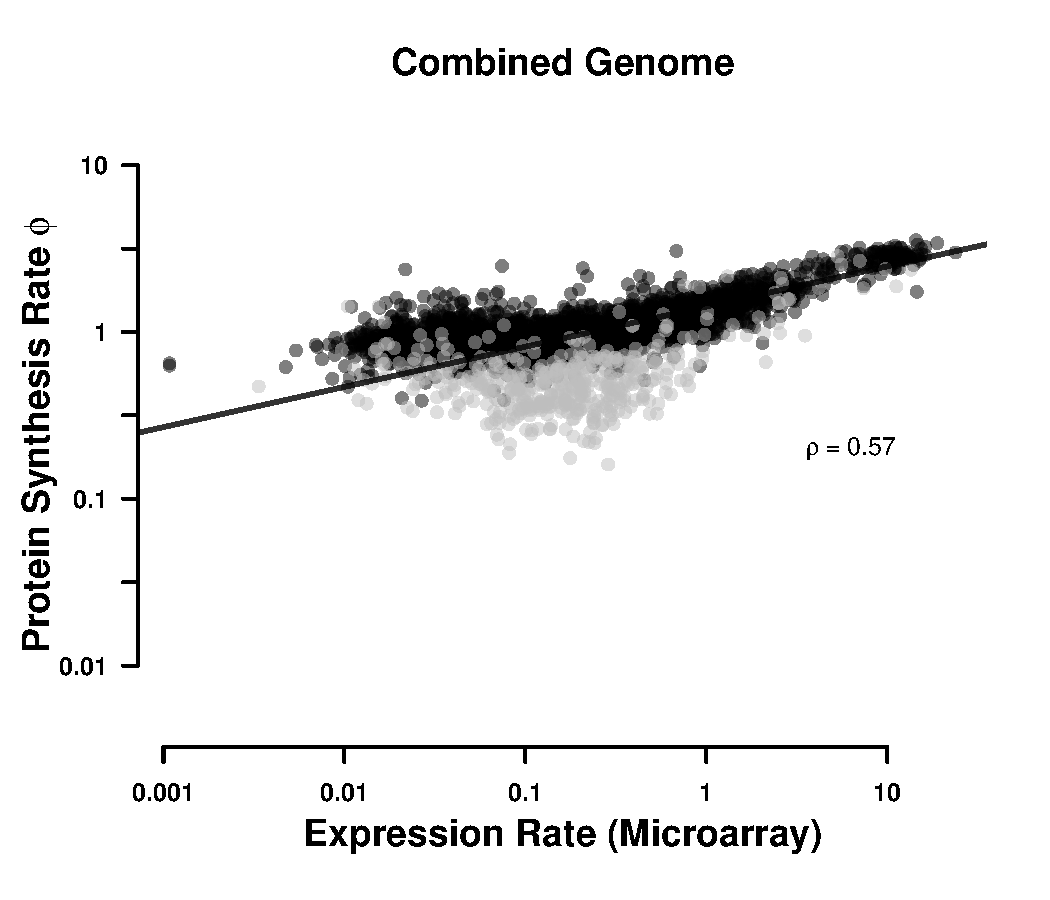
\includegraphics[width=.45\textwidth]{img/phi_corr_plot_whole_Genome_estim.pdf}
    \end{subfigure}
    \begin{subfigure}
        \centering
        (b) %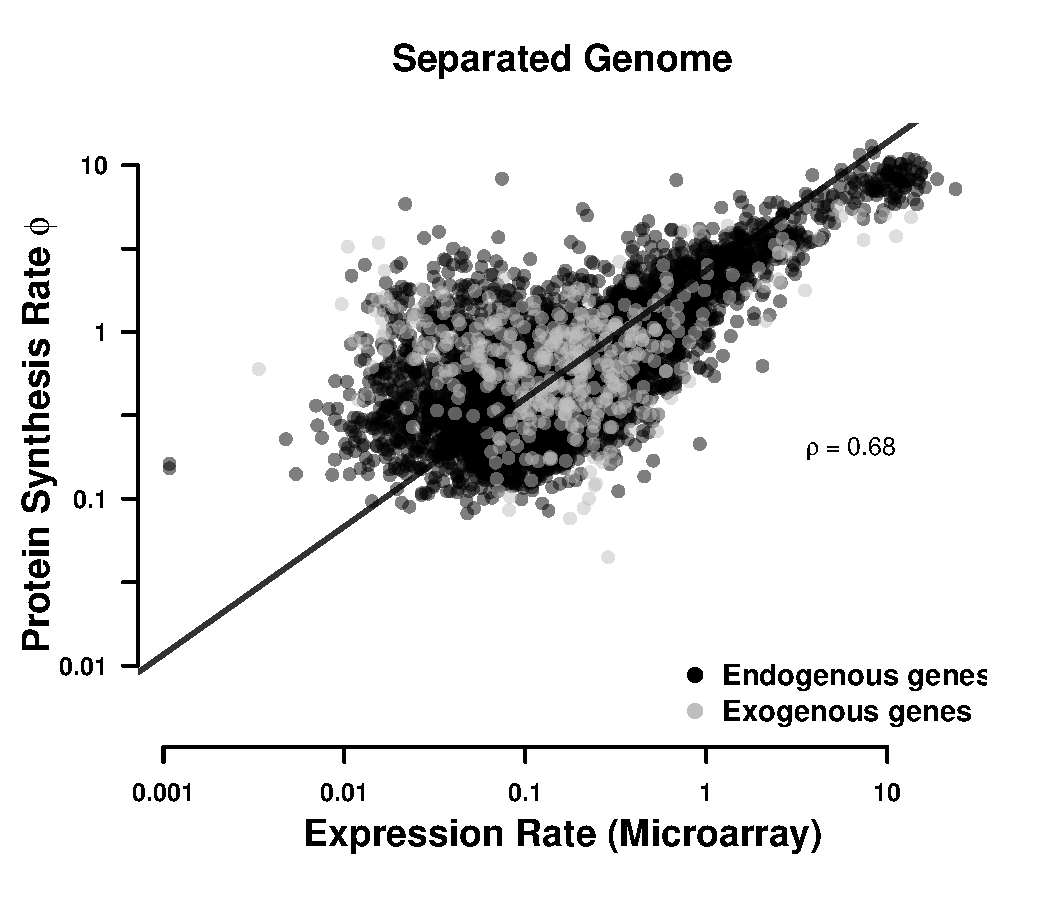
\includegraphics[width=.45\textwidth]{img/phi_corr_plot_split_Genome_estim.pdf}
    \end{subfigure}
    \caption{Comparison of predicted protein synthesis rate $\phi$ to microarray data from \citet{tsankov2010} for (a) the combined genome and (b) the separated endogenous and exogenous genes. 
    Endogenous genes are displayed in black and exogenous genes in red. 
    Black line indicates type II regression line assuming noise in the dependent and independent variable \citep{SokalAndRohlf1981}.}
    \label{fig:phi_corr_two_cond}
\end{figure}


\subsection*{Comparing Differences in the Endogenous and Exogenous Codon Usage}
To better understand the differences in the endogenous and exogenous cellular environments, we compared our parameter estimates of mutation bias \DM and selection \DE for the two sets of genes.
Our estimates of \DM for the endogenous and exogenous genes were negatively correlated ($\rho = -0.49$),  indicating weak similarity with only $\sim5\%$ of the codons share the same sign between the two mutation environments (Figure \ref{fig:csp_comp}a).
Overall, the endogenous genes only show a selection preference for C and G ending codons in $\sim58\%$ of the codon families.
In contrast, the exogenous genes display a strong preference for A and T ending codons in $\sim89\%$ of the codon families.

For example, the endogenous genes show a mutational bias for A and T ending codons in $\sim95\%$ of the codon families (the exception being Phe, F).
The exogenous genes display an equally consistent mutational bias towards C and G ending codons (Table \ref{tab:codon_pref_dm}).
%As a result, only the two codon amino acid Phenylalanine (Phe, F) shares the same rank order across the endogenous and exogenous \DM estimates.
In contrast to \DM, our estimates of \DE for the endogenous and exogenous genes were positively correlated ($\rho = 0.69$) and showing the same sign in $\sim53\%$ of codons between the two selection environments (Figure \ref{fig:csp_comp}).
\ROC constraints $E[\phi] = 1$, allowing us to interpret \DE as selection on codon usage of the average gene with $\phi = 1$ and gives us the ability to compare the efficacy of selection $s\Ne$  across genomes.

\begin{figure}
    \centering
    \begin{subfigure}
        \centering
        (a) %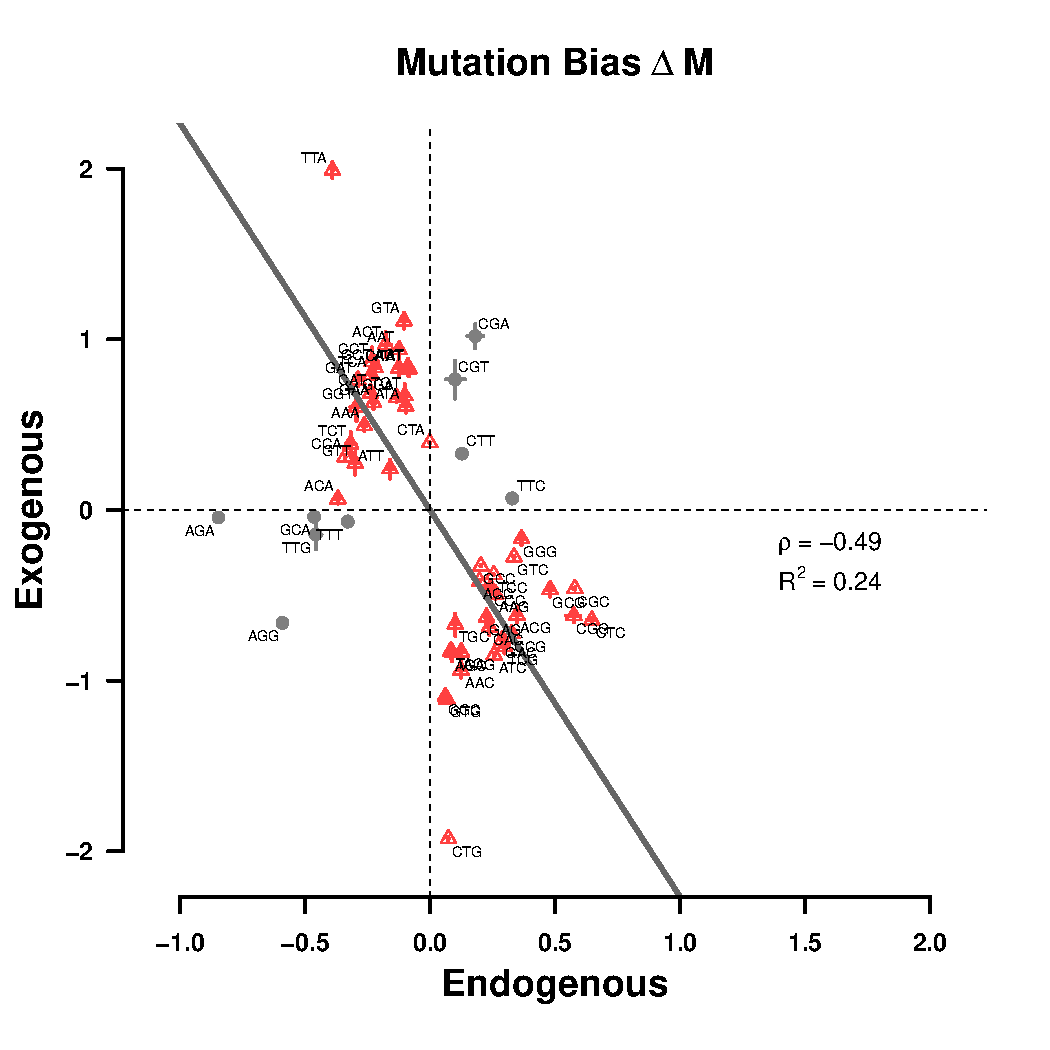
\includegraphics[width=.45\textwidth]{img/csp_corr_dm.pdf}
    \end{subfigure}
    \begin{subfigure}
        \centering
        (b) %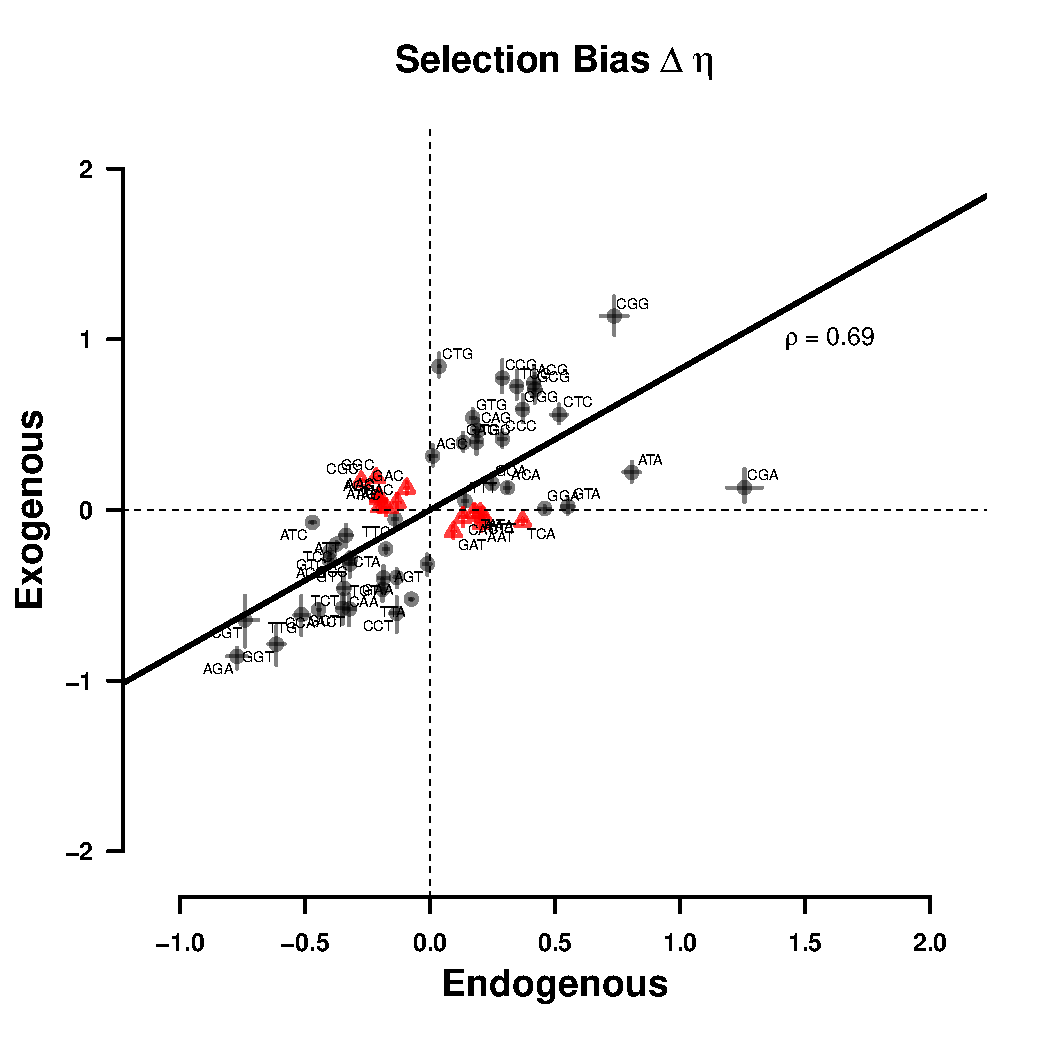
\includegraphics[width=.45\textwidth]{img/csp_corr_deta.pdf}
    \end{subfigure}
    \caption{Comparison of (a) mutation bias \DM and (b) selection bias \DE parameters for endogenous and exogenous genes.
      Estimates are relative to the mean for each codon family.
      Black dots indicate \DM or \DE parameters with the same sign for the endogenous and exogenous genes, red dots indicate parameters with different signs.
      Black line indicates type II regression line assuming noise in the dependent and independent variable \citep{SokalAndRohlf1981}.
      Dashed lines mark quadrants.}
    \label{fig:csp_comp}
\end{figure}


We find that the efficacy of selection within each codon family differs between sets of genes.
The difference in codon usage between endogenous and exogenous genes is striking as some amino acids have opposite codon preferences. 
As a result, our estimates of the optimal codon differ in nine cases between endogenous and exogenous genes (Figure \ref{fig:cub_endo_exo}, Table \ref{tab:codon_pref_deta}).
For example, the usage of the Asparagine (Asn, N) codon AAC is increased in highly expressed endogenous genes but the same codon is depleted in highly expressed exogenous genes.
For Aspartic acid (Asp, D), the combined genome shows the same codon preference in highly expressed genes as the exogenous gene set.
Generally, fits to the complete \kluyveri genome reveal that the relatively small exogenous gene set ($\sim 10\%$ of genes) has a disproportional effect on the model fit (Figure \ref{fig:cub_full_main}, \ref{fig:cub_full_cleft}).

Of the nine cases in which the endogenous and exogenous genes show differences in the selectively most favored codon five cases (Asp, D; His, H; Lys, K; Asn, N; and Pro, P) the endogenous genes favor the codon with the most abundant tRNA.
For the remaining four cases (Ile, I; Ser, S; Thr, T; and Val, V), there are no tRNA genes for the wobble free cognate codon encoded in the \kluyveri genome.
However, the codon preference of these four amino acids in the exogenous genes matches the most abundant tRNA encoded in the \kluyveri genome.

The effect of the small exogenous gene set on the fit to the complete \kluyveri genome is smaller in our estimates of selection bias \DE than \DM, but still large.
We find that the complete \kluyveri genome is estimated to share the selection preference with the exogenous genes in $\sim60\%$ of codon families that show dissimilarity between endogenous and exogenous genes.
We find that the complete \kluyveri genome fit shares mutational preference with the exogenous genes in $\sim78\%$ of the $19$ codon families showing a difference in mutational codon preference between the endogenous and exogenous genes.
In two cases, Isoleucine (Ile, I) and Arginine (Arg, R), the strong dissimilarity in mutation preference results in an estimated codon preference in the complete \kluyveri genome that differs from both the endogenous, and the exogenous genes.
These results clearly show that it is important to recognize the difference in endogenous and exogenous genes and treat these genes as separate sets to avoid the inference of incorrect synonymous codon preferences and better predict protein synthesis.

%D:GAC:T, H:CAC:T, I:ATT:FX, K:AAG:T, N:AAC:T, P:CCA:T, S:TCT:FX, T:ACT:FX, V:GTT:FX

\begin{figure}
     \centering
	%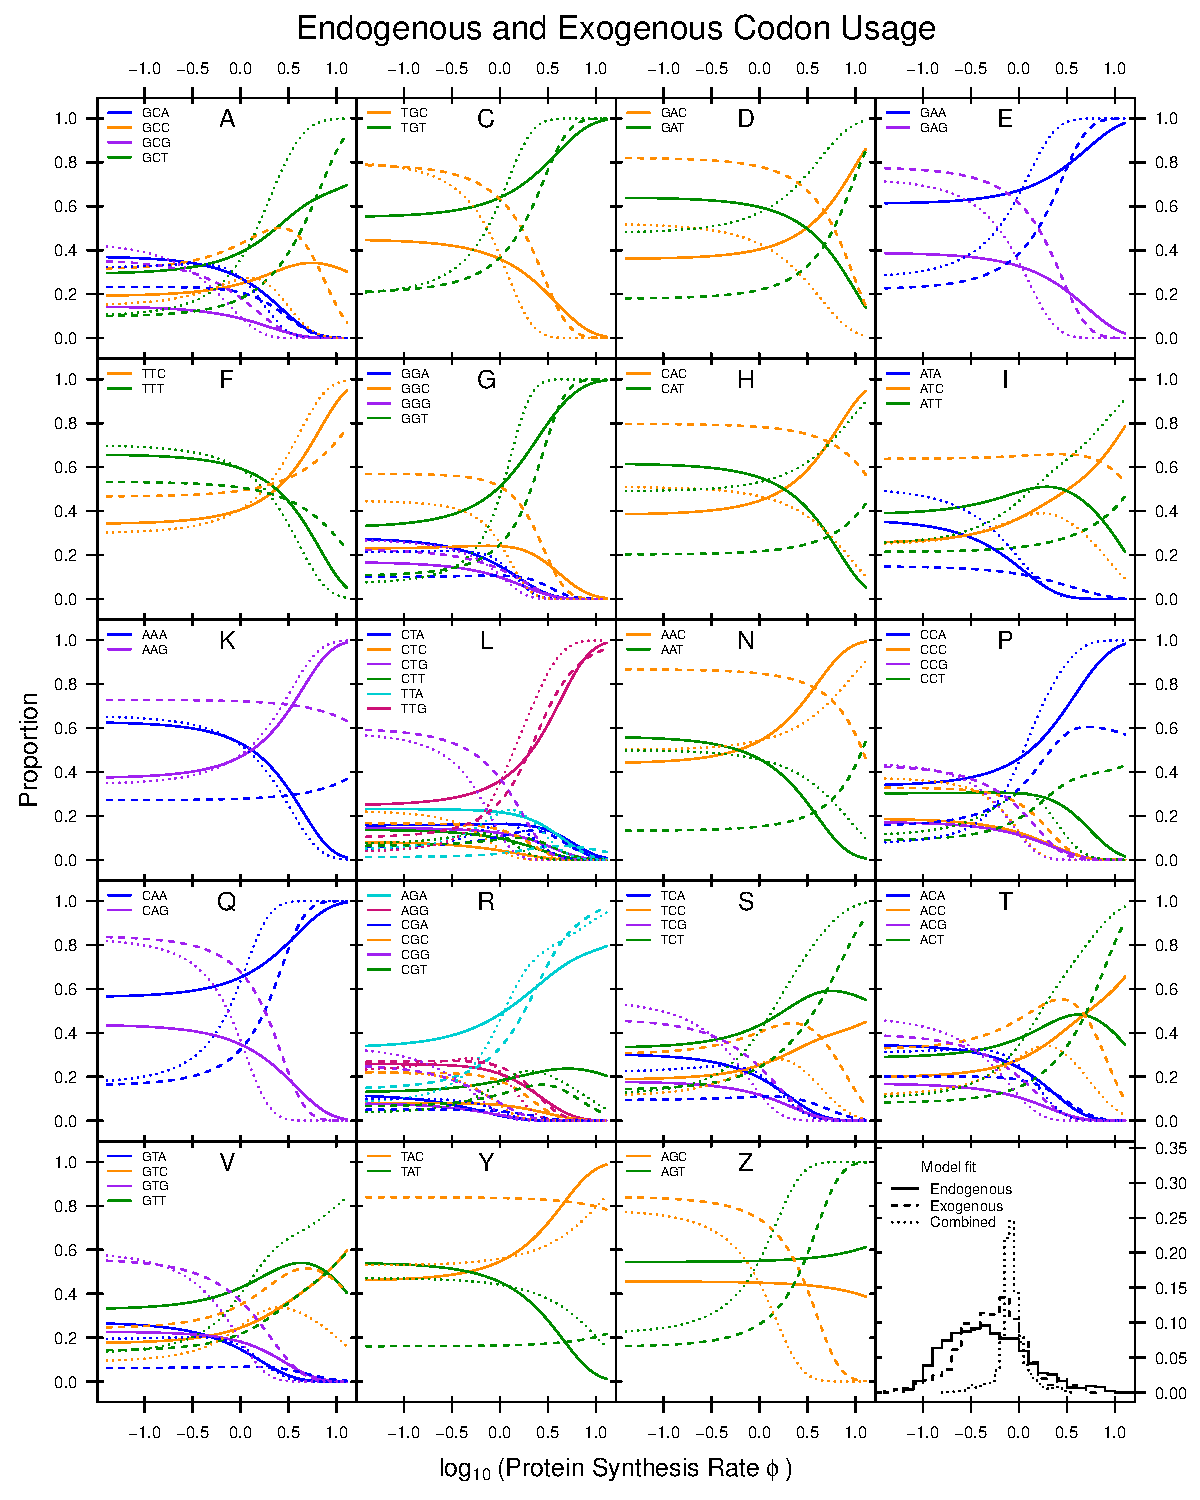
\includegraphics[width=\textwidth]{img/CUB_cleft_main.pdf}
	\caption{Codon usage patterns for 19 amino acids. Amino acids are indicated as one letter code. 
	The amino acids Serine was split into two groups (S and Z) as Serine is coded for by two groups of codons that are separated by more than one mutation.
	Solid line indicates the endogenous codon usage, dashed line indicates the exogenous codon usage.}
	\label{fig:cub_endo_exo}
\end{figure}



\subsection*{Determining Source of Exogenous Genes}

We combined our estimates of mutation bias \DM and selection bias \DE with synteny information and searched for potential source lineages of the introgressed exogenous region.
We examined 332 budding yeasts \citep{shen2018} and, identified the ten lineages with the highest correlation for the \DM parameters as potential source lineages (Figure \ref{fig:csp_exo_comp}, Table \ref{tab:source}).
We used \DM to identify candidate lineages as the endogenous and exogenous genes show greater dissimilarity in mutation bias than in selection bias.
Two of the ten candidate lineages utilize the alternative yeast nuclear code (NCBI codon table 12). 
In this case, the codon CTG codes for Serine instead of Leucine. 
We therefore excluded the Leucine codon family in our comparison of codon families, however, there was no need to exclude Serine as well as CTG is not a one step neighbor of the remaining Serine codons.
The endogenous \kluyveri genome exhibits codon usage very similar to most (77 \%) yeast lineages examined, indicating that most of the examined yeasts share a similar codon usage (Figure \ref{fig:csp_endo_comp}).
Only $\sim 17 \%$ of all examined yeast show a positive correlation in both, \DM and \DE with the exogenous genes, whereas the vast majority of lineages ($\sim 83 \%$) show a negative correlation for \DM, only 21 \% show a negative correlation for \DE.
%This indicates that information on mutation bias provides more information about a potential origin of the exogenous genes.

\begin{table}
  \centering
  \caption{Budding yeast lineages showing similarity in codon usage with the exogenous genes.
  $\rho_\DM$ and $\rho_\DE$ represent the Pearson correlation coefficient for \DM and \DE, respectively.
  \GC is the average \GC of the whole genome.
  Synteny is the percentage of the exogenous genes found in the listed lineage.
  Only one lineage (\gossypii) shows a similar \GC $> 50 \%$.}
  \begin{threeparttable}
  	\begin{tabular}{lcccccc}
    		\hline
    		Species & $\rho_\DM$ & $\rho_\DE$ & \GC & Synteny \%&  Distance [Mya] \\ \hline 
    		\emph{Eremothecium gossypii}			& 0.89 & 0.70 & 51.7 & 75 & 211.0847 \\
    		\emph{Danielozyma ontarioensis}			& 0.75 & 0.92 & 46.6 & 3   & 470.1043 \\
    		\emph{Metschnikowia shivogae}			& 0.86 & 0.87 & 49.8 & 0   & 470.1043 \\
    		%\emph{Metschnikowia aberdeeniae}		& 0.74 & 0.88 & 48.5 & 0   & 470.1043 \\
    		\emph{Babjeviella inositovora}			& 0.83 & 0.78 & 48.1 & 0   & 470.1044 \\
    		\emph{Ogataea zsoltii}					& 0.75 & 0.85 & 47.7 & 0   & 470.1042 \\ 
    		\emph{Metschnikowia hawaiiensis}		& 0.80 & 0.86 & 44.4 & 0   & 470.1042 \\
    		%\emph{Candida tenuis}					& 0.74 & 0.86 & 43.0 & 0   & 470.1044 \\
    		\emph{Candida succiphila}	       			& 0.85 & 0.83 & 40.9 & 0   & 470.1042 \\ 
    		\emph{Middelhovenomyces tepae}		& 0.80 & 0.62 & 40.8 & 0   & 651.9618 \\ 
    		\emph{Candida albicans*}		   		& 0.84 & 0.75 & 33.7 & 0   & 470.1043 \\
    		%\emph{Candida tammaniensis}			& 0.66 & 0.80 & 33.5 & 0   & 470.1043 \\
   		\emph{Candida dubliniensis*}               		& 0.78 & 0.75 & 33.1 & 0   & 470.1043 \\ \hline
  	\end{tabular}
  	\begin{tablenotes}
    		\item[*] Lineages use the alternative yeast nuclear code % check how to reference NCBI codon table numbers
 	 \end{tablenotes}
  \end{threeparttable}  
  \label{tab:source}
\end{table}

Comparing synteny between the exogenous genes, which are restricted to the left arm of chromosome C, and the determined candidate yeast species we find that \gossypii is the only species that displays high synteny (Table \ref{tab:source}).
Furthermore, the synteny relationship between the exogenous region and other yeasts appears to be limited to Saccharomycetaceae clade.
Given these results, we conclude that of the 332 examined yeast lineages the \gossypii lineage is the most likely source of the introgressed exogenous genes.
This result is in contrast to previous studies which studied the exogenous genes and chromosome recombination in the Lachancea clade and concluded that the exogenous region originated from within the Lachancea clade \citep{payen2009, friedrich2015, vakirlis2016}.
To validate our results, we identified 121 genes in our dataset \citep{shen2018} with homologous gene in \gossypii and \textit{L. thermotolerance} and used IQTree \citep{nguyen2015} to infer the phylogenetic relationship of the exogenous genes. Our results show that $\sim 60 \%$ of exogenous genes (73/121) are more closely related to \gossypii than to other Lachancea.
Interestingly, our results also indicate that codon usage does not necessarily correlate with phylogenetic distance (Table \ref{tab:source}). 

\begin{figure}
     \centering
	%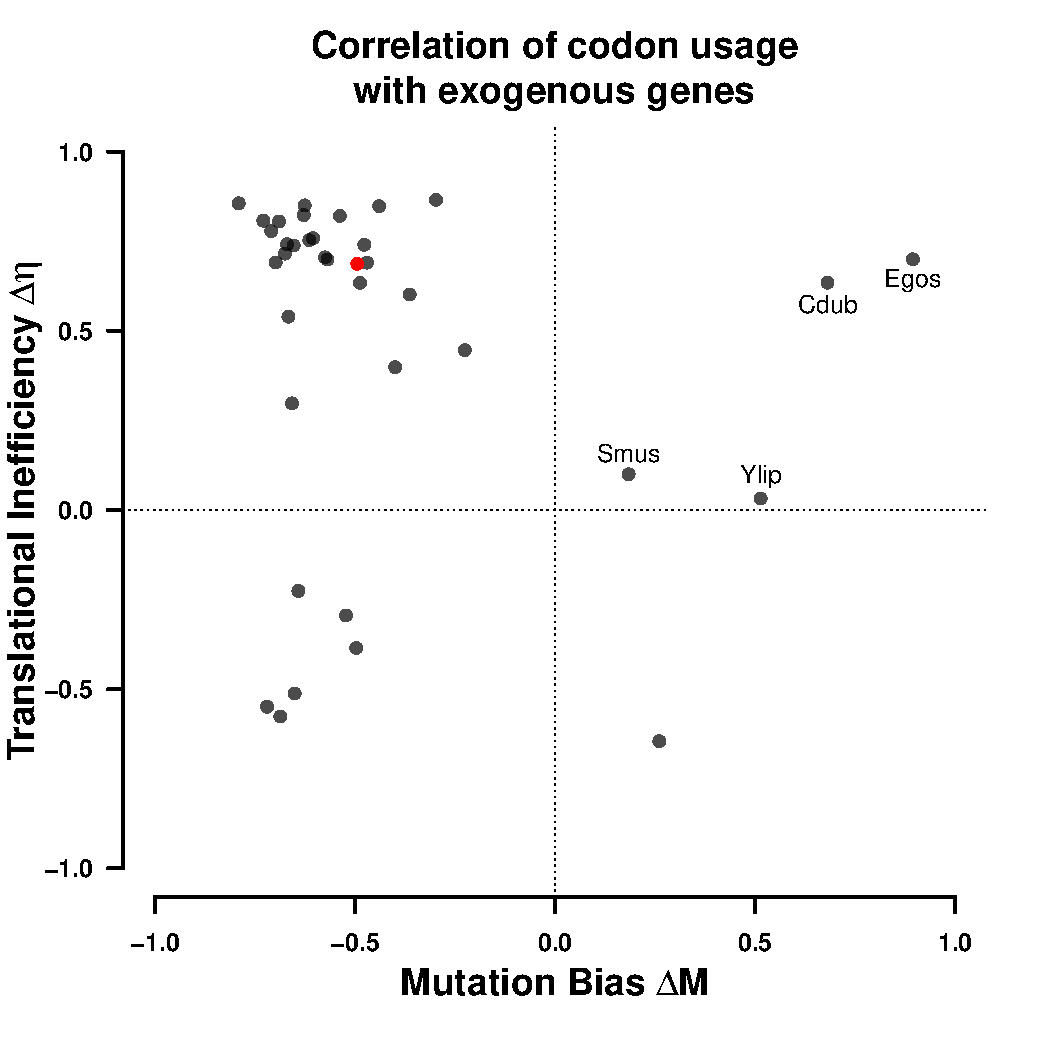
\includegraphics[width=.45\textwidth]{img/csp_mean_correlation_exo.pdf}
	\caption{Correlation coefficients of \DM and \DE of the exogenous genes with 332 examined budding yeast lineages. 
	Dots indicate the correlation of \DM and \DE of the lineages with the exogenous parameter estimates.
	Blue triangles indicate the \textit{Lachancea} and red diamonds indicate \textit{Eremothecium} species.
	All regressions were performed using a type II regression assuming noise in the dependent and independent variable \citep{SokalAndRohlf1981}.}
	\label{fig:csp_exo_comp}
\end{figure}


\subsection*{Estimating Introgression Age}

We modeled the change in codon frequency over time as exponential decay, and estimated the age of the introgression assuming that \gossypii still represents the mutation bias of its ancestral source lineage at the time of the introgression and a constant mutation rate.
We infer the age of the introgression to be on the order of $6.2\pm1.2\times 10^8$ generations. 
Assuming \kluyveri experiences between one and eight generations per day, we estimate the introgression to have occurred between $212,000$ to $1,700,000$ years ago.
Our estimate places the time of the introgression earlier than the previous estimate of 19,000 - 150,000 years by \citet{friedrich2015}.

Using our model of exponential decay model, we also estimated the persistence of the signal of the exogenous cellular environment.
%We assume that differences in mutation bias will decay more slowly than differences in selection bias to be able to utilize our bias free estimates of \DM.
We predict that the \DM signal of the source cellular environment will have decayed to be within one percent of the \kluyveri environment in $\sim 5.4\pm0.2\times 10^9 $ generations, or between $1,800,000$ and $15,000,000$ years.
Together, these results indicate that the mutation signature of the exogenous genes will persist for a very long time.

\subsection*{Estimating Selection against Codon Mismatch of the Exogenous Genes}

We define the selection against inefficient codon usage as the difference between the fitness on the log scale of an expected, replaced endogenous gene and the exogenous gene, $s \propto \phi \DE$ due to the mismatch in codon usage parameters (See Methods for details).
As the introgression occurred before the diversification of \kluyveri and has fixed throughout all populations \citep{friedrich2015}, we can not observe the original endogenous sequences that have been replaced by the introgression.
Overall, we predict that a small number of low expression genes ($\phi < 1$) were weakly exapted at the time of the introgression (Figure \ref{fig:sne_fitness_burden}a).
High expression genes ($\phi > 1$) are predicted to have faced the largest selection against their mismatched codon usage in the novel cellular environment.
In order to account for differences in the efficacy of selection on codon usage either due to the cost of pausing, differences in the effective population size, or the decline in fitness with every ATP wasted between the donor lineage and \kluyveri we added a linear scaling factor $\kappa$ to scale our estimates of \DE between the donor lineage and \kluyveri and searched for the value that minimized the cost of the introgression, thus giving us the best case scenario (See Methods for details).



Using our estimates of $\Delta M$ and $\Delta \eta$ from the endogenous genes and assuming the current exogenous amino acid composition of genes is representative of the replaced endogenous genes, we estimate the selection against the exogenous genes at the time of introgression (Figure \ref{fig:sne_fitness_burden}a) and currently (Figure \ref{fig:sne_fitness_burden}b).
Estimates of selection bias for the exogenous genes show that, while well correlated with the endogenous genes, only nine amino acids share the same selectively preferred codon.
Exogenous genes are, therefore, expected to represent a significant reduction in fitness for \kluyveri due to mismatch in codon usage.
We estimate that the selection against the exogenous genes due to mismatched codon usage to have been $\GL \approx -0.0008$ at the time of the introgression and $\approx -0.0003$ today.
This reduction in $\GL$ is primarily due to adaptive changes to the codon usage of the most highly expressed, introgressed genes (Figures \ref{fig:sne_fitness_burden}a \& \ref{fig:adapt_tot}).
Based on the selection against the codon mismatch at the time of the introgression and assuming an effective population size $\Ne$ on the order of $10^7$ \citep{wagner2005}, we approximate a fixation probability of $(1-\exp[-\GL])/(1-\exp[-2\GL \Ne]) \approx 10^{-6952}$ \citep{SellaAndHirsh2005} for the exogenous genes.
Clearly, the possibility of fixation under this simple scenario is effectively zero (See Discussion).



\begin{figure}
    \centering
    \begin{subfigure}
        \centering
        (a) %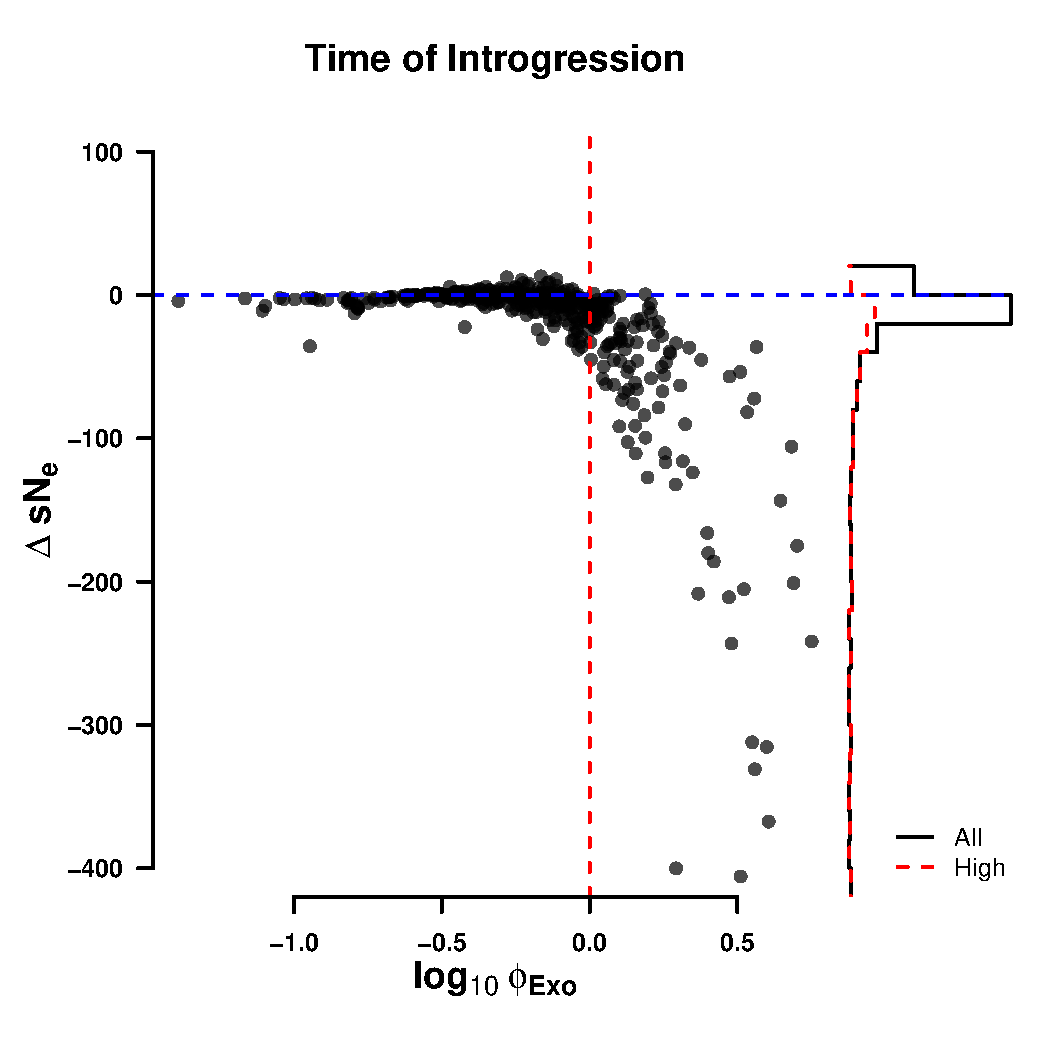
\includegraphics[width=.45\textwidth]{img/fitness_difference_gos_kappa5.pdf}
    \end{subfigure}
    \begin{subfigure}
        \centering
        (b) %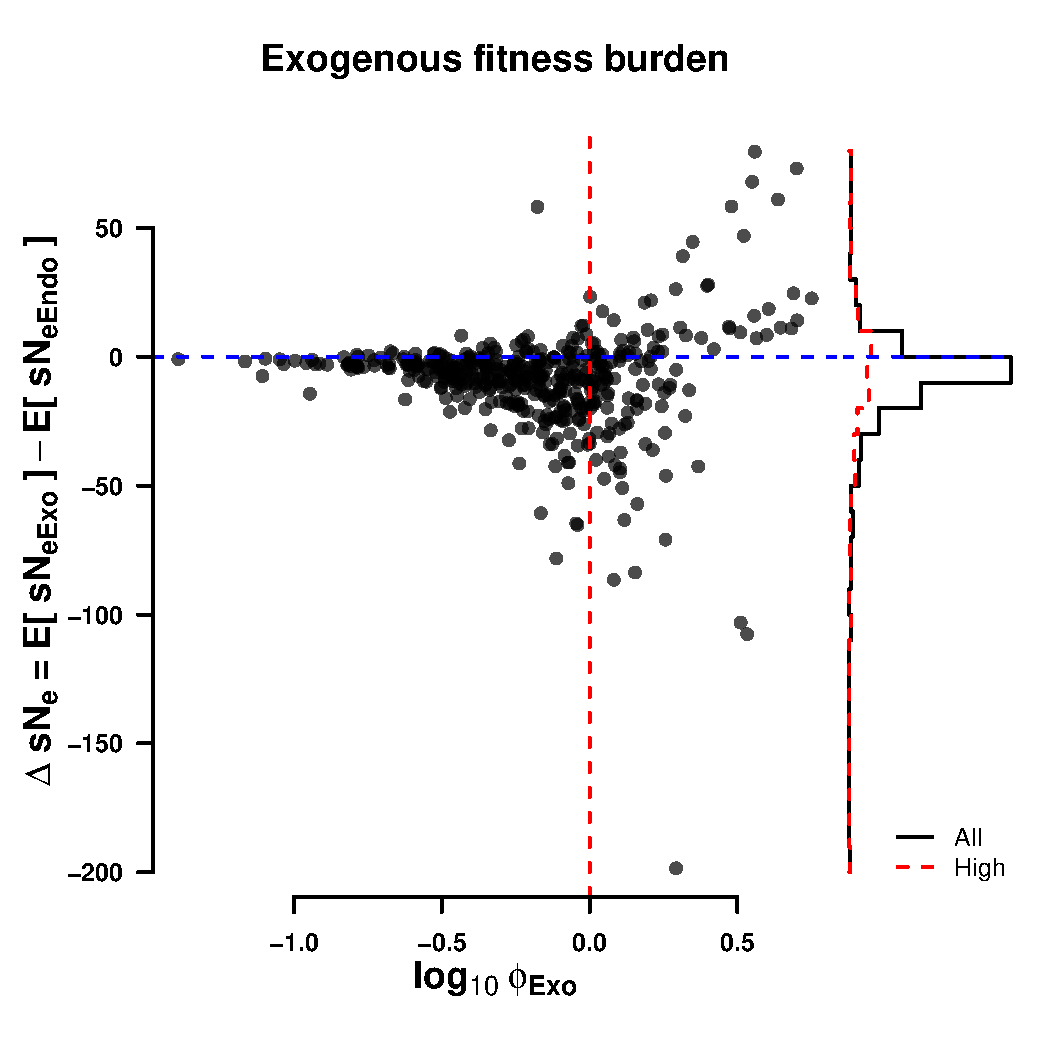
\includegraphics[width=.45\textwidth]{img/fitness_difference_exo.pdf}
    \end{subfigure}
    \caption{Selection against mismatched codon usage $s = \DE \phi$ (a) at the time of introgression ($\kappa = 5$), and (b) currently ($\kappa = 1$). 
        Vertical dashed line indicates split between high and low expression genes at $\phi = 1$.
    	Horizontal dashed line indicates neutrality.}
    \label{fig:sne_fitness_burden}
\end{figure}


\section*{Discussion}
In order to study the evolutionary effects of the large scale introgression of the left arm of chromosome C, we used \ROC, a mechanistic model of ribosome movement along an mRNA.
The usage of a mechanistic model rooted in population genetics allows us generate more nuanced quantitative parameter estimates and separate the effects of mutation and selection on the evolution of codon usage.
This allowed us to calculate the selection against the introgression, and provides \gossypii as a potential source lineage of the introgression which was previously not considered.
Our parameter estimates indicate that the \kluyveri genome contains distinct signatures of mutation and selection bias from both an endogenous and exogenous cellular environment.
By fitting \ROC separately to \kluyveri's endogenous and exogenous sets of genes we generate a quantitative description of their signatures of mutation bias and natural selection for efficient protein translation.

Previous work by \cite{payen2009} showed an increased preference for GC rich codons in the exogenous genes but our results provide more nuanced insights by separating the effects of mutation bias and selection.
We are able to show that the difference in \GC between endogenous and exogenous genes is mostly due to differences in mutation bias as 95\% of exogenous codon families show a strong mutation bias towards GC ending codons (Table \ref{tab:codon_pref_dm}).
However, the exogenous genes show a selective preference for AT ending codons for 90\% of codon families (Table \ref{tab:codon_pref_deta}).
Acknowledging the increased mutation bias towards GC ending codons and the difference in strength of selection between endogenous and exogenous genes by separating them also improves our estimates of protein synthesis rate $\phi$ by $42 \%$ relative to the full genome estimate ($R^2 = 0.46$ vs.~$0.32$, respectively).

The mutation and selection bias parameters \DM and \DE of the introgressed exogenous genes contain information, albeit decaying, about its previous cellular environment.
We selected the top ten lineages with the highest similarity in \DM to see if our parameters estimates would allow us to identify a potential source lineage.
The synteny relationship of these lineages with the exogenous genes was calculated as a point of comparison as it provides orthogonal information to our parameter estimates.
Synteny with the exogenous genes is limited to the Saccharomycetaceae clade, excluding all of the potential source lineages identified using codon usage but \gossypii (Table \ref{tab:source}).
Interestingly, this also showed that similarity in codon usage does not correlate with phylogenetic distance.

Previous work indicated that the donor lineage of the exogenous genes has to be a, potentially unknown, Lachancea lineage \citep{payen2009, friedrich2015, vakirlis2016, brion2017}.
These previous results, however, are based on species rather than genes trees ignoring the differential adaptation rate to their novel cellular environment between genes or due not consider lineages outside of the Lachancea clade.
Considering the similarity in selection bias (Figure \ref{fig:csp_comp}b) and our calculation of selection on the exogenous genes (Figure \ref{fig:sne_fitness_burden}b), both of which are free of any assumption about the origin of the exogenous genes, a species tree estimated from the exogenous genes may be biased towards the Lachancea clade.
Estimating individual gene trees rather than relying on a species tree provided further evidence that the exogenous genes could originate from a lineage that does not belong to the Lachancea clade.
As we highlighted in this study, relatively small sets of genes with a signal of a foreign cellular environment can significantly bias the outcome of a study. 
The same holds true for phylogenetic inferences \citep{salichos2013}, and as we showed the signal of the original endogenous cellular environment that shaped CUB is at different stages of decay in high and low expression genes (Figure \ref{fig:adapt_tot}).
In summary, our work does not dispute an unknown Lachancea as possible origin, but provides an alternative hypothesis based on the codon usage of the exogenous genes, phylogenetic analysis, and synteny.

In terms of understanding the spread of the introgression, we calculated the expected selective cost of codon mismatch between the \kluyveri and \gossypii lineages.
Under our working hypothesis, the majority of the introgressed would have imposed a selective cost due to codon mismatch.
Nevertheless, $\sim 30 \%$ of low expression exogenous genes ($\phi < 1$) appeared to be exapted at the time of the introgression.
This exaptation is due to the mutation bias in the endogenous genes matching the selection bias in the exogenous genes for GC ending codons.
Our estimate of the selective cost of codon mismatch on the order of $-0.0008$.
While this selective cost may not seem very large, assuming \kluyveri had a large \Ne, the fixation probability of the introgression is the astronomically small value of $\approx 10^{-6952} \approx 0$.
Thus, the basic scenario of an introgression between two yeast species with large \Ne and where the introgression solely imposes a selective cost due to codon mismatch is clearly too simplistic.

For example, one or more loci with a combined selective advantage on the order of $0.0008$ or greater would have made the introgression change from disadvantageous to effectively neutral or advantageous.
While this scenario seems plausible, it raises the question as to why recombination events did not limit the introgression to only the adaptive loci.
A potential answer is the low recombination rate between the endogenous and exogenous regions \cite{payen2009, brion2017}.
This is presumably due to the dissimilarity in \GC and/or a lower than average sequence homology between the exogenous region and the one it replaced.
A population bottleneck reducing the \Ne of the \kluyveri lineage around the time of the introgression could also help explain the spread of the introgression.
Compatible with these explanation is the possibility of several advantageous loci distributed across the exogenous region drove a rapid selective sweep and/or the population through a bottleneck speciation process.


Assuming \gossypii as potential source lineage of the exogenous region, we illustrated how information on codon usage can be used to infer the time since the introgression occurred using our estimates of mutation bias \DM.
The \DM estimates are well suited for this task as they are free of the influence of selection and unbiased by $\Ne$ and other scaling terms, which is in contrast to our estimates of \DE \citep{gilchrist2015}.
Our estimated age of the introgression of $6.2\pm1.2\times 10^8$ generations is $\sim 10$ times longer than a previous minimum estimate by \cite{friedrich2015} of $5.6\times 10^7$ generations, which was based on the effective population recombination rate and the population mutation parameter \citep{Ruderfer2006}.
Furthermore, these estimates assume that the current \gossypii and \kluyveri cellular environment reflect their ancestral states at the time of the introgression.
Thus, if the ancestral mutation environments were more similar (dissimilar) at the time of the introgression then our result is an overestimate (underestimate).

\section*{Conclusion}
Overall, our results show the usefulness of the separation of mutation bias and selection bias and the importance of recognizing the presence of multiple cellular environments in the study of codon usage.
We also illustrate how a mechanistic model like \ROC and the quantitative estimates it provides can be used for more sophisticated hypothesis testing in the future.
In contrast to other approaches used to study codon usage like CAI \citep{sharp1987} or tAI \citep{dosreis2004}, \ROC incorporates the effects of mutation bias and amino acid composition explicitly \citep{cope2018}.
We highlight potential issues when estimating codon preferences, as estimates can be biased by the signature of a second, historical cellular environment.
In addition, we show how quantitative estimates of mutation bias and selection relative to drift can be obtained from codon data and used to infer the fitness cost of an introgression as well as its history and potential future.

\section*{Materials and Methods}

\subsection*{Separating Endogenous and Exogenous Genes}
A GC-rich region was identified by \cite{payen2009} in the \kluyveri genome extending from position 1 to 989,693 of chromosome C.
This region was later identified as an introgression by \cite{friedrich2015}.
We obtained the \kluyveri genome from SGD Project \url{http://www.yeastgenome.org/download-data/} (on 09-27-2014) and the annotation for \kluyveri NRRL Y-12651 (assembly ASM14922v1) from NCBI (on 12-09-2014).
We assigned 457 genes located on chromosome C with a location within the $\sim 1$ Mb window to the exogenous gene set.
All other 4864 genes of the \kluyveri genome were assigned to the exogenous genes.

\subsection*{Model Fitting with \ROC}
\ROC was fitted to each genome using AnaCoDa (0.1.1) \citep{landerer2018} and R (3.4.1) \citep{rcore}.
\ROC was run from 10 different starting values for at least 250,000 iterations and thinned to every 50th iteration.
After manual inspection to verify that the MCMC had converged, parameter posterior means, log posterior probability and log likelihood were estimated from the last 500 samples (last 10\% of samples).

\subsection*{Model selection}
The marginal likelihood of the combined and separated model fits was calculated using a generalized harmonic mean estimator \citep{Gronau2017}. A variance scaling of 1.1 was used to scale the important density of the estimator. Using the estimated marginal likelihoods, we calculated the Bayes factor to assess model performance. 
Increases in the variance scaling increase the estimated Bayes factor, therefore we report a conservative Bayes factor bases on a small variance scaling \ref{fig:bf_scaling}.

\subsection*{Comparing Codon Specific Parameter Estimates and Selecting Candidate lineages}
As the choice of reference codon can reorganize codon families coding for an amino acid relative to each other, all parameter estimates were interpreted relative to the mean for each codon family.
\begin{equation}
\DM_i = \DM_{i,1} - \overline{\DM_i}
\end{equation}
\begin{equation}
\DE_i = \DE_{i,1} - \overline{\DE_i}
\end{equation}
Comparison of codon specific parameters (\DM and $\DE = 2\Ne q(\eta_i-\eta_j)$) was performed using the function lmodel2 in the R package lmodel2 (1.7.3) \citep{lmodel2} and R version 3.4.1 \citep{rcore}.
The parameter \DE can be interpreted as the difference in fitness between codon $i$ and $j$ for the average gene with $\phi = 1$ scaled by the  effective population size $\Ne$, and the selective cost of an ATP $q$ \citep{gilchrist2007, gilchrist2015}.
Type II regression was performed with re-centered parameter estimates, accounting for noise in dependent and independent variable \citep{SokalAndRohlf1981}.

Due to the greater dissimilarity of the \DM estimates between the endogenous and exogenous genes, and the slower decay rate of mutation bias, we decided to focus on our estimates of mutation bias to identify potential source lineages.
The top ten lineages with the highest similarity in \DM to the exogenous genes were selected as potential candidates (Figure \ref{fig:csp_comp}).

\subsection*{Phylogenetic Analysis}
Using the dataset from \cite{shen2018}, we first identified 121 alignments for exogenous genes and further contained homologous genes for \gossypii, and \textit{L. thermotolerance}.
We excluded all species from the alignments that do not belong to the Saccharomycetaceae clade. 
IQTree \citep{nguyen2015} was used to identify the best fitting model for each gene and to estimate the individual gene trees.
The distance between \kluyveri, \gossypii, and \textit{L. thermotolerance} was calculated for each tree to identify genes for which exogenous genes are more closely related to \gossypii or  \textit{L. thermotolerance}.

\subsection*{Synteny Comparison}
We obtained complete genome sequences for all 10 candidate lineages (Table \ref{tab:source}) from NCBI (on: 02-05-2017).
Genomes were aligned and checked for synteny using SyMAP (4.2) with default settings \citep{soderlund2006, soderlund2011}.
We assess synteny as percentage coverage of the exogenous gene region.

\subsection*{Estimating Age of Introgression}
We modeled the change in codon frequency over time using an exponential model for all two codon amino acids, and describing the change in codon $c_1$ as
\begin{equation}
\frac{d c_1}{d t} = -\mu_{1,2}c_1 - \mu_{2,1}(1-c_1)
\label{mut_ode}
\end{equation}
where $\mu_{i,j}$ is the rate at which codon $i$ mutates to codon $j$ and $c_1$ is the frequency of the reference codon.
Initial codon frequencies $c_1(0)$ for each codon family where taken from our mutation parameter estimates for \gossypii where $c_1(0) = \exp[\DM_\text{gos}]/(1+\exp[\DM_\text{gos}])$. 
Our estimates of $\DM_\text{endo}$ can be used to calculate the steady state of equation \ref{mut_ode} were $\frac{d c_1}{d t} = 0$ to obtain the equality
\begin{equation}
\frac{\mu_{2,1}}{\mu_{1,2} + \mu_{2,1}} = \frac{1}{1+\exp[\DM_\text{endo}]}
\end{equation}
Solving for $\mu_{1,2}$ gives us $\mu_{1,2} = \DM_\text{endo}\exp[\mu_{2,1}]$ which allows us to rewrite and solve equation \ref{mut_ode} as
\begin{equation}
c_1(t) = \frac{ 1 + \exp[-X](K-1) }{ 1+\DM_\text{endo} }
\label{mut_close_form}
\end{equation}
where $X = (1+\DM_\text{endo})\mu_{2,1}t$ and $K = c_1(0)(1+\DM_\text{endo}) $.

Equation \ref{mut_close_form} was solved with a mutation rate $\mu_{2,1}$ of $3.8\times 10^{-10}$ per nucleotide per generation \citep{lang2008}. 
Current codon frequencies for each codon family where taken from our estimates of \DM from the exogenous genes.
Mathematica (11.3) \citep{Mathematica11} was used to calculate the time $t_\text{intro}$ it takes for the initial codon frequencies $c_1(0)$ for each codon family to equal the current exogenous codon frequencies.
The same equation was used to determine the time $t_\text{decay}$ at which the signal of the exogenous cellular environment has decayed to within $1 \%$ of the endogenous environment.

\subsection*{Estimating Selection against Codon Mismatch}

In order to estimate the selection against codon mismatch, we had to make three key assumptions.
First, we assumed that the current exogenous amino acid sequence of a gene is representative of its ancestral state and the replaced endogenous gene it replaced.
Second, we assume that the currently observed cellular environment of \gossypii reflects the cellular environment that the exogenous genes experienced before transfer to \kluyveri.
Lastly, we assume that the difference in the efficacy of selection between the cellular environments due to differences in either effective population size $\Ne$ or the selective cost of an ATP $q$ of the source lineage and \kluyveri can be expressed as a scaling constant and that protein synthesis rate $\phi$ has not changed between the replaced endogenous and the introgressed exogenous genes.
Using estimates for $\Ne = 1.36\times10^7$ \citep{wagner2005} for \textit{Saccharomyces paradoxus} we scale our estimates of \DE which explicitly contains the effective population size $\Ne$ \citep{gilchrist2015} and define $\DE' = \frac{\DE}{\Ne}$.

All of our genome parameter estimations are scaled by lineage specific effects such as \Ne, the average, absolute gene expression level, and/or the proportionate fitness value of an ATP.
In order to account for these genome specific differences in scaling, we scale the difference in the efficacy of selection on codon usage between the donor lineage and \kluyveri using a linear scaling factor $\kappa$.
As \DE is defined as $\DE = 2\Ne q(\eta_i-\eta_j)$, we cannot distinguish if $\kappa$ is a scaling on protein synthesis rate $\phi$, effective population size $\Ne$, or the selective cost of an ATP $q$ \citep{gilchrist2007, gilchrist2015}.
We calculated the selection against each genes codon mismatch assuming additive fitness effects as 
\begin{equation}
s_g = \sum_{i=1}^{L_g} -\kappa \phi_g \DE'_i
\label{equ:sg}
\end{equation}
where $s_g$ is the overall strength of selection for translational efficiency on gene, $g$  in the exogenous gene set, $\kappa$ is a constant, scaling the efficacy of selection between the endogenous and exogenous cellular environments, $L_{g}$ is length of the protein in codons, $\phi_g$ is the estimated protein synthesis rate of the gene in the endogenous environment, and $\DE'_i$, is the $\DE'$ for the codon at position $i$.
As stated previously, our \DE are relative to the mean of the codon family.
We find that the selection against the introgressed genes is minimized at $\kappa \sim 5$ (Figure \ref{fig:sne_scaling}b).
Thus, we expect a five fold difference in the efficacy of selection between \kluyveri and \gossypii, due to differences in either protein synthesis rate $\phi$, effective population size $\Ne$, and/or the selective cost of an ATP $q$.
Therefore, we set $\kappa = 1$ if we calculate the $s_g$ for the endogenous and the current exogenous genes, and $\kappa = 5$ for $s_g$ for selection calculations at the time of introgression.

However, since we are unable to observe codon sequences of the replaced endogenous genes and for the exogenous genes at the time of introgression, instead of summing over the sequence, we calculate the expected codon count $E[n_{g,i}] $ for codon $i$ in gene $g$ simply as the probability of observing codon $i$ multiplied by the number of times the corresponding amino acids is observed in gene $g$, yielding:
\begin{align*}
E[n_{g,i}] &= P(c_i | \DM, \DE, \phi) \times m_{a_i}\\
 &= \frac{\exp[-\DM_i -\DE_i\phi_g]}{\sum_j^C \exp[-\DM_j -\DE_j\phi_g]}\times m_{a_i}
\end{align*} 
where $m_{a_i}$ is the number of occurrences of amino acid $a$ that codon $i$ codes for.
Thus replacing the summation over the sequence length $L_g$ in equ. (\ref{equ:sg}) by a summation over the codon set $C$ and calculating $s_g$ as
\begin{equation}
s_g = \sum_{i=1}^{C} -\kappa \phi_g \DE'_i E[n_{g,i}] 
\end{equation}
We report the selection due to mismatched codon usage of the introgression as $\GL_g = s_{\text{intro},g} - s_{\text{endo},g}$ where $s_{\text{intro},g}$ is the selection against an introgressed gene $g$ either at the time of the introgression or presently.


\begin{backmatter}
  
\section*{Acknowledgments}
The authors would like to thank Alexander Cope for helpful criticisms and suggestions for this work.

\section*{Availability of data and materials}
Parameter estimates generated during this study are available from the corresponding author.
All remaining data generated during this study are included in this published article as figures, tables.

\section*{Authors' contributions}
CL and MAG initiated the study.
CL collected and analyzed the data and wrote the manuscript.
MAG and BCO edited the manuscript.
CL, MAG, BCO, and RZ contributed to the data analysis and acquiring of funding.
All Authors approved the final manuscript.
    
\section*{Funding}
This work was supported in part by NSF Awards MCB-1120370 (MAG and RZ),  MCB-1546402 (A. Von Arnim and MAG), and DEB-1355033 (BCO, MAG, and RZ) with additional support from Department of Ecology \& Evolutionary Biology (EEB) at the University of Tennessee Knoxville (UTK) and  the National Institute for Mathematical and Biological Synthesis (NIMBioS), an Institute sponsored by the National Science Foundation through NSF Award DBI-1300426.
CL received support as a Graduate Student Fellow from NIMBioS with additional support from Departments of Mathematics and EEB at UTK. 

\section*{Ethics approval and consent to participate}
Not applicable

\section*{Consent for publication}
Not applicable

\section*{Competing interests}
The authors declare that they have no competing interests.



\bibliographystyle{bmc-mathphys} 
%\bibliographystyle{natbib}
\bibliography{kluyveri_paper}


\clearpage
%\pagebreak



\suppl

%%% commands for getting SM pages and figures labeled with S
%% different than with other .cls
\setcounter{section}{19} %appendix environment set in .cls file.  Set this to 19 to get an 'S' for figures
\setcounter{page}{1}
\renewcommand{\thepage}{S\arabic{page}} %this works

\section*{Supplementary Material}
%\beginsupplement

Supporting Materials for \emph{Unlocking a signal of introgression from codons in Lachancea kluveri using a mutation-selection model} \ by Landerer \emph{et al.}.

\begin{table}[h]
    \centering
    \caption{Synonymous mutation codon preference based on our estimates of $\DM$.
	 Shown are the most likely codon in low expression genes for each amino acid in: \gossypii, in the endogenous and exogenous genes of \kluyveri, and in the combined \kluyveri genome without accounting for the two cellular environments.}
\begin{tabular}{  l  c  c  c  c  }
\hline
	Amino Acid & \gossypii & Endogenous & Exogenous & Combined \\ \hline
	Ala A & GCG & GCA & GCG & GCG \\ 
	Cys C & TGC & TGT & TGC & TGC \\ 
	Asp D & GAC & GAT & GAC & GAC \\ 
	Glu E & GAG & GAA & GAG & GAG \\ 
	Phe F & TTC & TTT & TTT & TTT \\ 
	Gly G & GGC & GGT & GGC & GGC \\ 
	His H & CAC & CAT & CAC & CAC \\ 
	Ile I & ATC & ATT & ATC & ATA \\ 
	Lys K & AAG & AAA & AAG & AAA \\ 
	Leu L & CTG & TTG & CTG & CTG \\ 
	Asn N & AAC & AAT & AAC & AAT \\ 
	Pro P & CCG & CCA & CCG & CCG \\ 
	Gln Q & CAG & CAA & CAG & CAG \\ 
	Arg R & CGC & AGA & AGG & CGG \\ 
	Ser$_4$ S & TCG & TCT & TCG & TCG \\
	Thr T & ACG & ACA & ACG & ACG \\ 
	Val V & GTG & GTT & GTG & GTG \\ 
	Tyr Y & TAC & TAT & TAC & TAC \\ 
	Ser$_2$ Z & AGC & AGT & AGC & AGC \\ \hline
\end{tabular}
    \label{tab:codon_pref_dm}
\end{table}

\clearpage

\begin{table}
    \centering
    \caption{Synonymous selection codon preference based on our estimates of $\DE$.
	 Shown are the most likely codon in high expression genes for each amino acid in: \gossypii, in the endogenous and exogenous genes of \kluyveri, and in the combined \kluyveri genome without accounting for the two cellular environments.}
\begin{tabular}{  l  c  c  c  c  }
\hline
	Amino Acid & \gossypii & Endogenous & Exogenous & Combined \\ \hline
	Ala A & GCT & GCT & GCT & GCT \\ 
	Cys C & TGT & TGT & TGT & TGT \\ 
	Asp D & GAT & GAC & GAT & GAT \\ 
	Glu E & GAA & GAA & GAA & GAA \\ 
	Phe F & TTT & TTC & TTC & TTC \\ 
	Gly G & GGA & GGT & GGT & GGT \\ 
	His H & CAT & CAC & CAT & CAT \\ 
	Ile I & ATA & ATC & ATT & ATT \\ 
	Lys K & AAA & AAG & AAA & AAG \\ 
	Leu L & TTA & TTG & TTG & TTG \\ 
	Asn N & AAT & AAC & AAT & AAC \\ 
	Pro P & CCA & CCA & CCT & CCA \\ 
	Gln Q & CAA & CAA & CAA & CAA \\ 
	Arg R & AGA & AGA & AGA & AGA \\ 
	Ser$_4$ S & TCA & TCC & TCT & TCT \\ 
	Thr T & ACT & ACC & ACT & ACT \\ 
	Val V & GTT & GTC & GTT & GTT \\ 
	Tyr Y & TAT & TAC & TAT & TAC \\ 
	Ser$_2$ Z & AGT & AGT & AGT & AGT \\ \hline
\end{tabular}
    \label{tab:codon_pref_deta}
\end{table}
\clearpage


\begin{figure}
     \centering
	%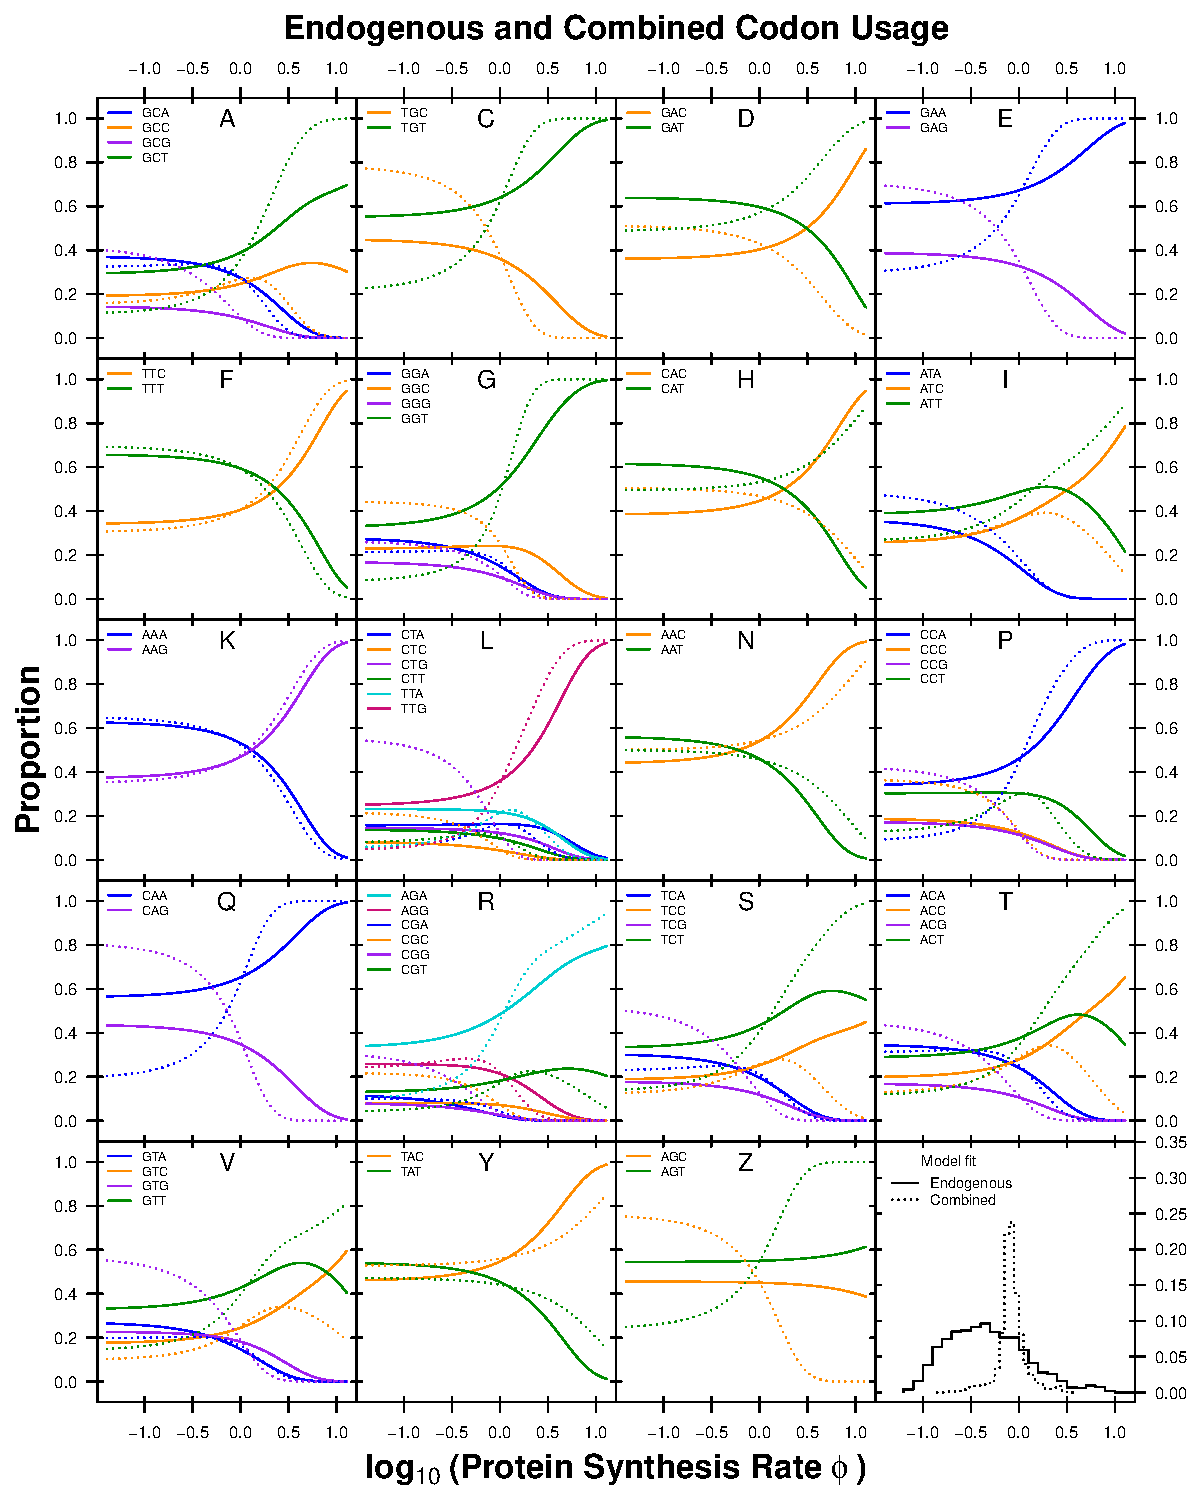
\includegraphics[width=\textwidth]{img/CUB_full_main.pdf}
	\caption{Codon usage patterns for 19 amino acids. Amino acids are indicated as one letter code. 
	The amino acids Serine was split into two groups (S and Z) as Serine is coded for by two groups of codons that are separated by more than one mutation.
	Solid line indicates the endogenous codon usage, dotted line indicates the combined codon usage.}
	\label{fig:cub_full_main}
\end{figure}
\null
\vfill
\begin{figure}
     \centering
	%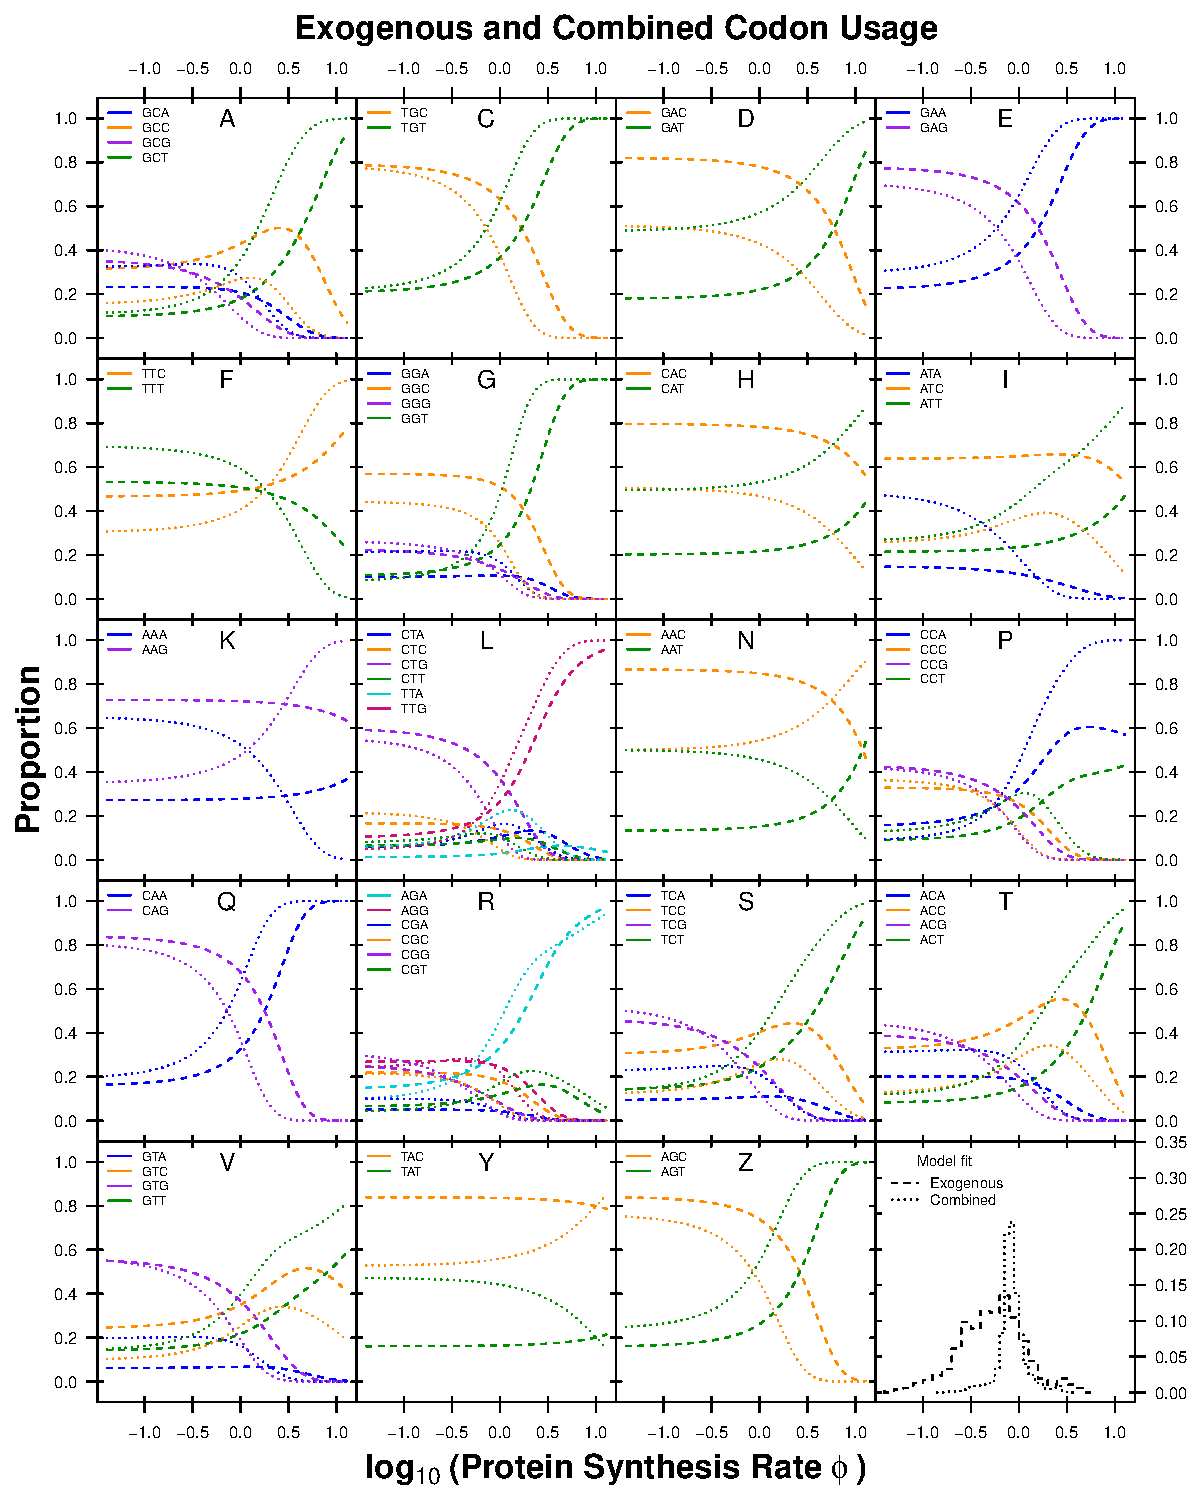
\includegraphics[width=\textwidth]{img/CUB_full_cleft.pdf}
	\caption{Codon usage patterns for 19 amino acids. Amino acids are indicated as one letter code. 
	The amino acids Serine was split into two groups (S and Z) as Serine is coded for by two groups of codons that are separated by more than one mutation.
	dashed line indicates the exogenous codon usage, dotted line indicates the combined codon usage.}
	\label{fig:cub_full_cleft}
\end{figure}

\null
\vfill
\begin{figure}
     \centering
	%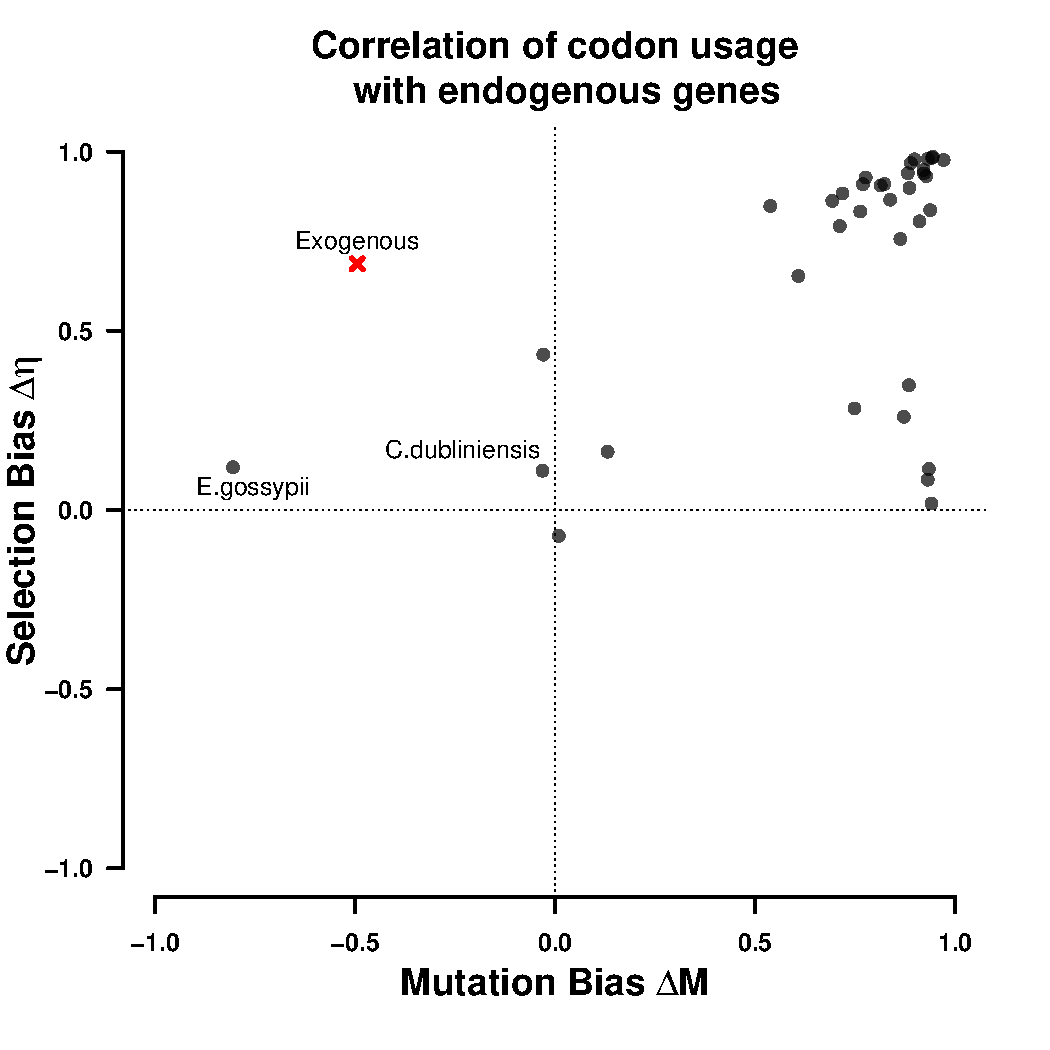
\includegraphics[width=0.5\textwidth]{img/csp_mean_correlation_endo.pdf}
	\caption{Correlation coefficients of \DM and \DE of the endogenous genes with 332 examined budding yeast lineages. 
	Dots indicate the correlation of \DM and \DE of the lineages with the exogenous parameter estimates.
	Blue triangles indicate the Lachancea and red diamonts indicate Eremothecium lineages.
	All regressions were performed using a type II regression assuming noise in the dependent and independent variable \citep{SokalAndRohlf1981}.}
	\label{fig:csp_endo_comp}
\end{figure}
\null
\vfill
\clearpage


\begin{figure}
    \centering
    \begin{subfigure}
        \centering
       % 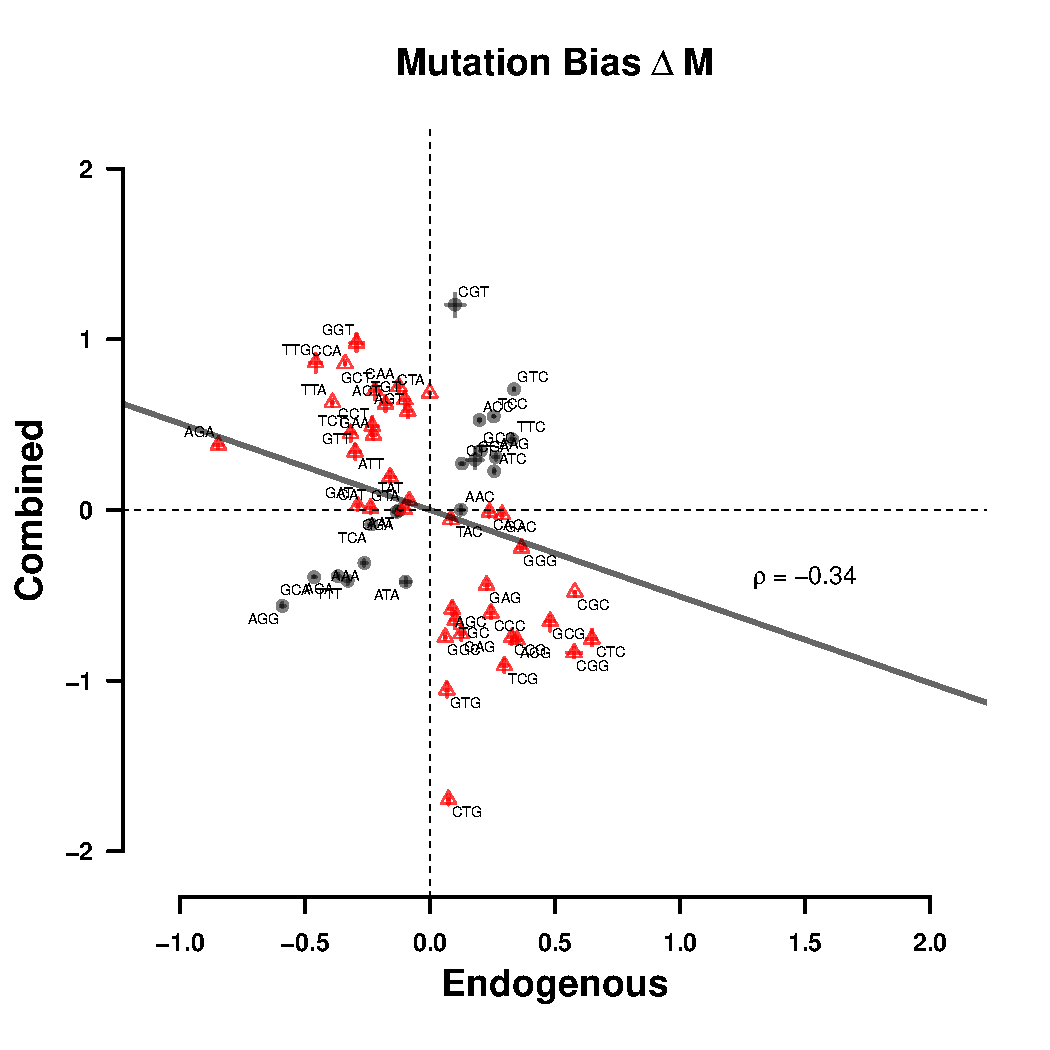
\includegraphics[width=.45\textwidth]{img/csp_corr_dm_full.pdf}
    \end{subfigure}
    \begin{subfigure}
        \centering
        %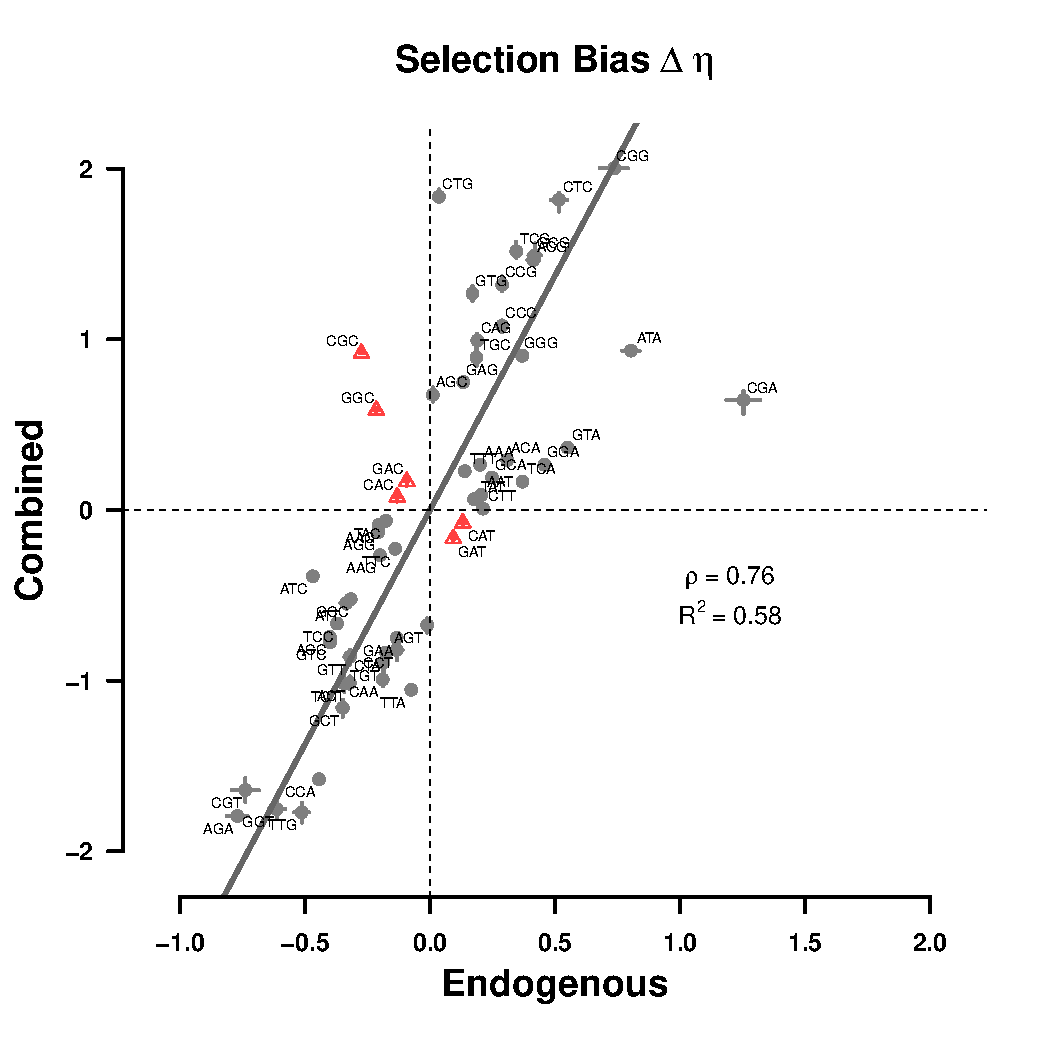
\includegraphics[width=.45\textwidth]{img/csp_corr_deta_full.pdf}
    \end{subfigure}
    \caption{Comparison of (a) mutation bias \DM and (b) selection bias \DE parameters for endogenous genes and combined gene sets.
      Estimates are relative to the mean for each codon family.
      Black dots indicate \DM or \DE parameters with the same sign for the endogenous and exogenous genes, red dots indicate parameters with different signs.
      Black line indicates type II regression line assuming noise in the dependent and independent variable \citep{SokalAndRohlf1981}.
      Dashed lines mark quadrants.}
    \label{fig:csp_end_comb}
\end{figure}
\null
\vfill
\clearpage

\begin{figure}
    \centering
    \begin{subfigure}
        \centering
       % 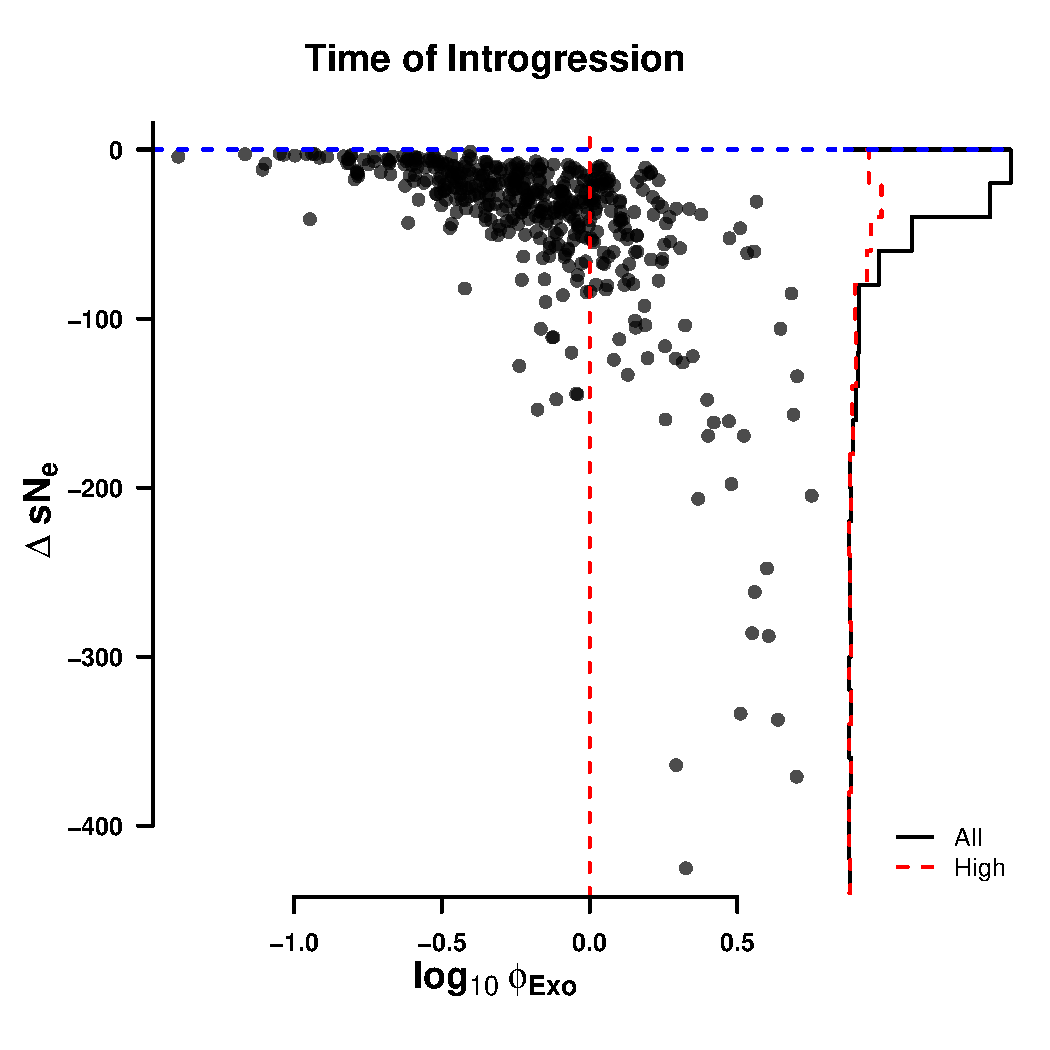
\includegraphics[width=.45\textwidth]{img/fitness_difference_gos_kappa1.pdf}
    \end{subfigure}
    \begin{subfigure}
        \centering
        %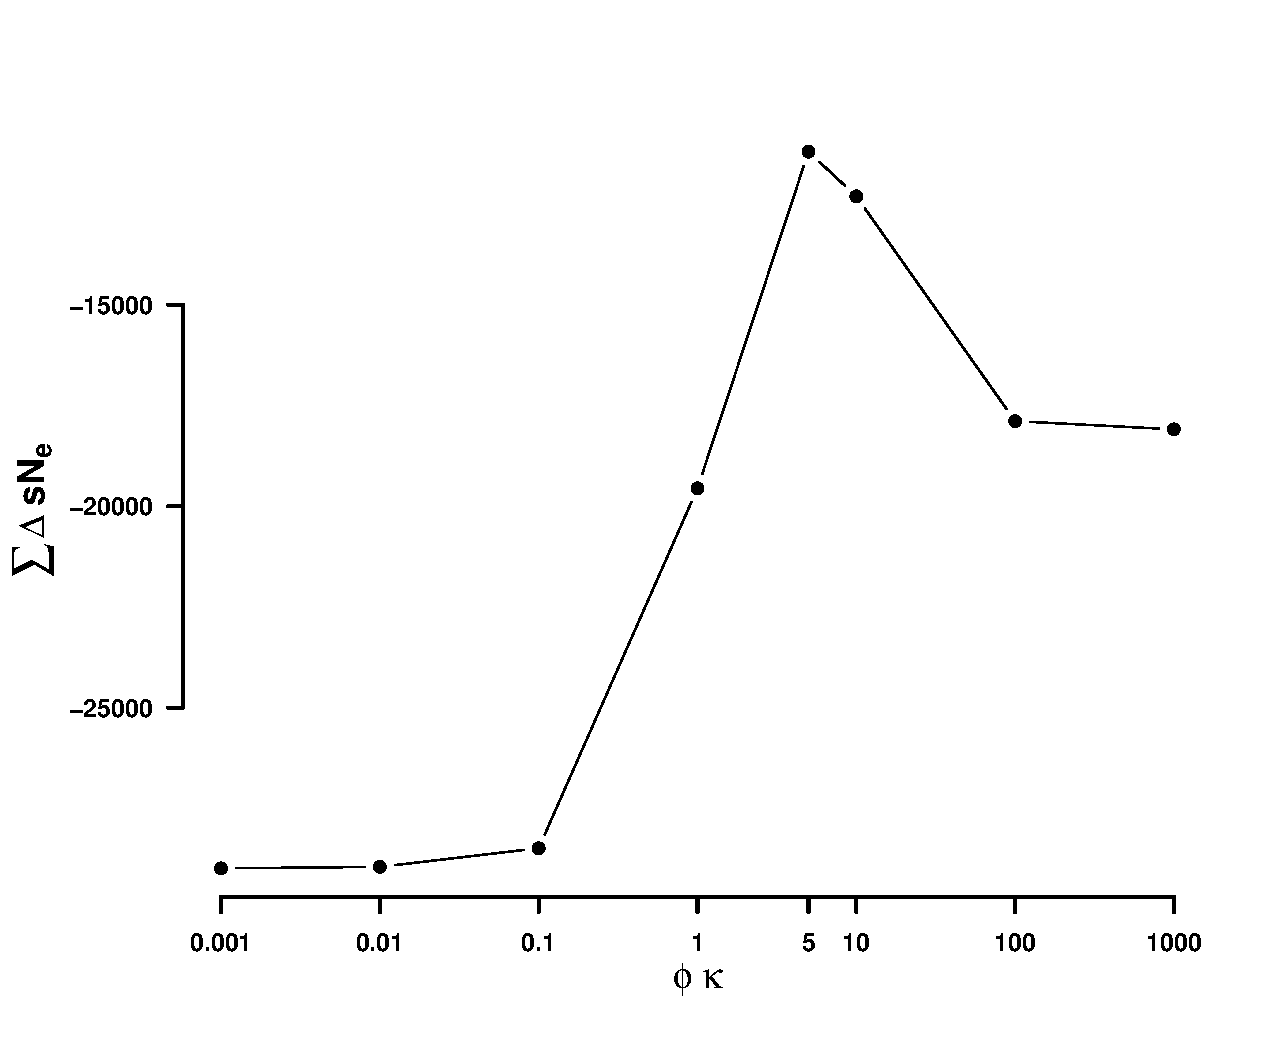
\includegraphics[width=.45\textwidth]{img/fitness_phi_scaling_gos.pdf}
    \end{subfigure}
    \caption{Selection against mismatched codon usage (left) without scaling of $\phi$ per gene. 
    Vertical dashed line indicates split between high and low expression genes at $\phi = 1$.
    Horizontal dashed line indicates neutrality.
     (Right) Change of total selection against mismatched codon usage with scaling term $\kappa$ between \gossypii and \kluyveri}
    \label{fig:sne_scaling}
\end{figure}
\null
\vfill
\clearpage
\null
\vfill
\begin{figure}
     \centering
	%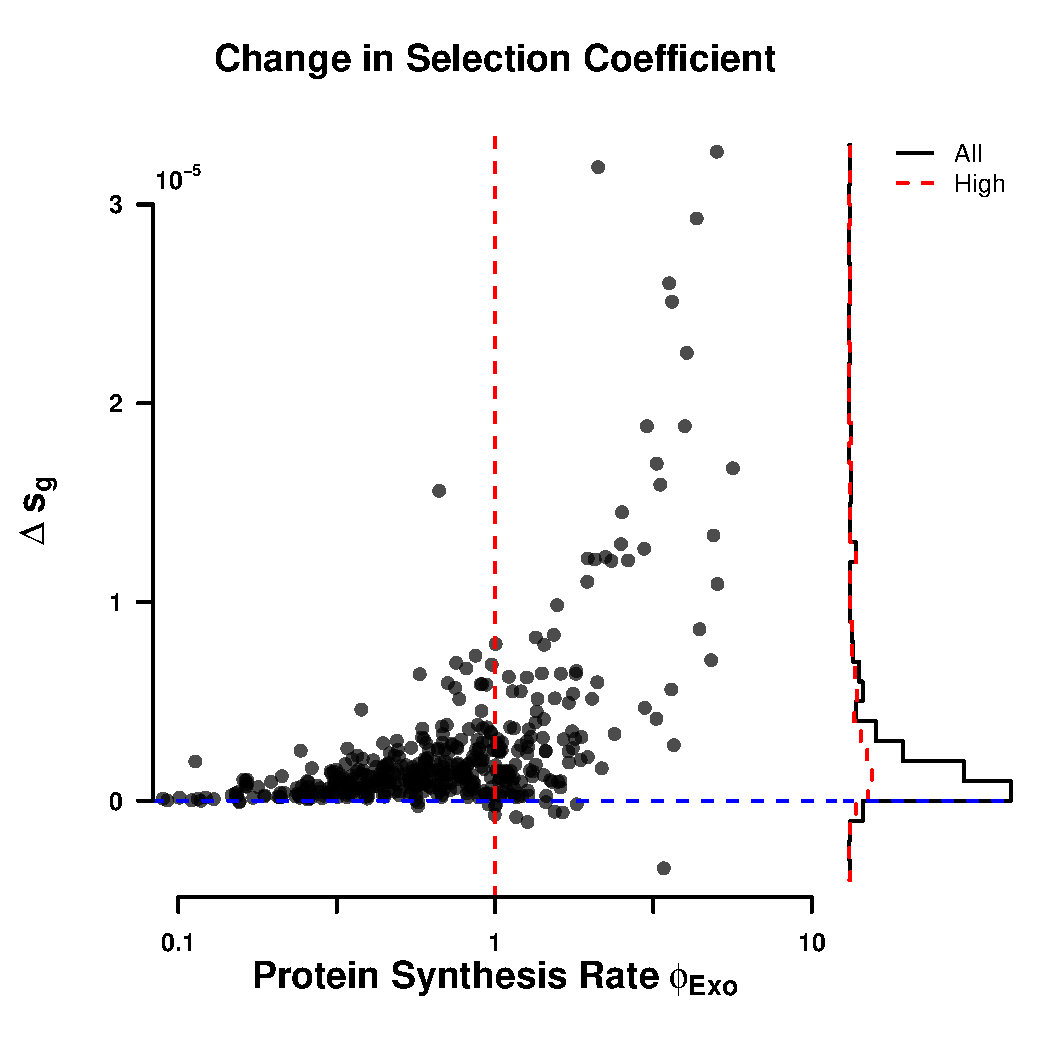
\includegraphics[width=.5\textwidth]{img/adaptation_total.pdf}
	\caption{Total amount of adaptation estimated to have occurred between time of introgression and currently observed per gene.
	    Vertical dashed line indicates split between high and low expression genes at $\phi = 1$.
	    Horizontal dashed line indicates no change in selection against mismatched codon usage.}
	\label{fig:adapt_tot}
\end{figure}
\null
\vfill
\clearpage
\null
\vfill
\begin{figure}
     \centering
	%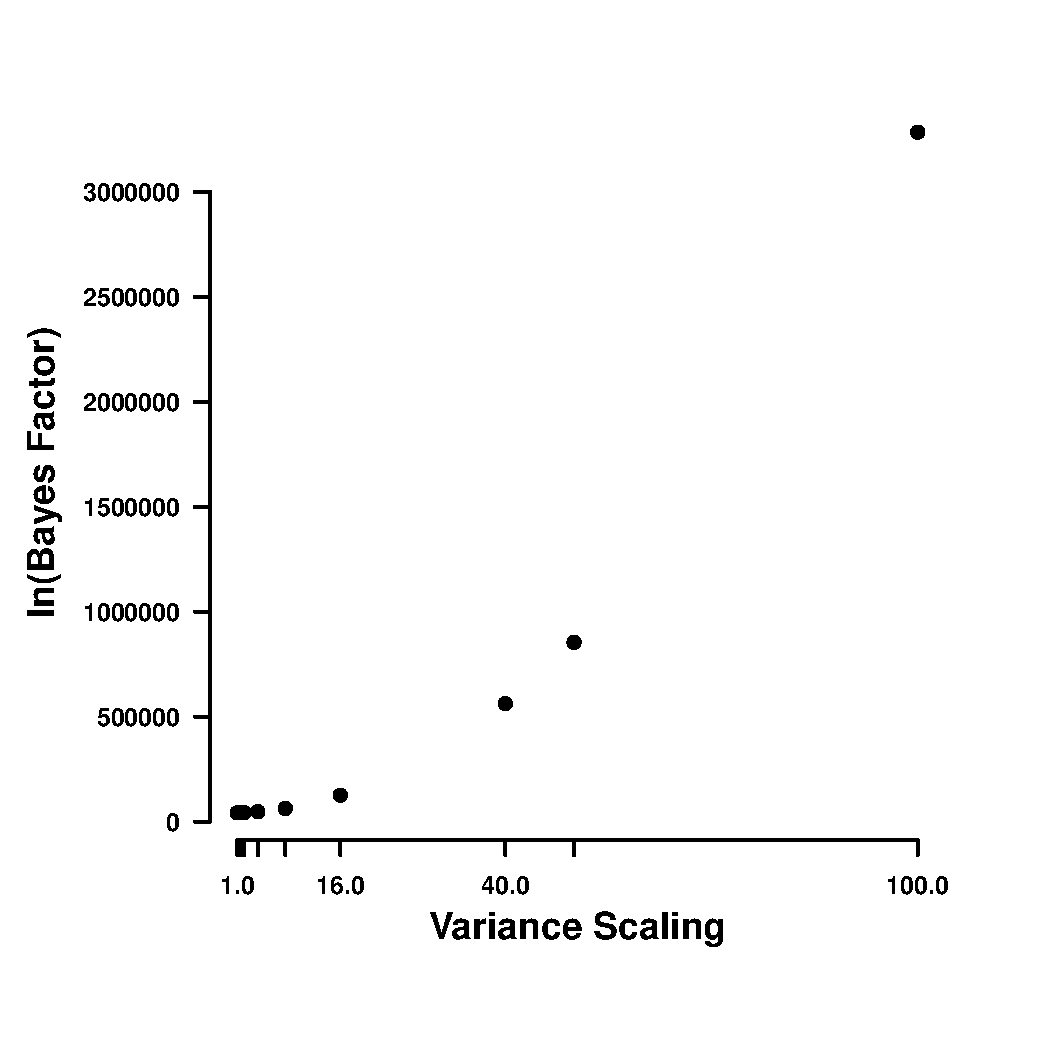
\includegraphics[width=.5\textwidth]{img/bf_variance_scaling.pdf}
	\caption{Influence of the variance scaling of the importance distribution on the estimated Bayes factor.}
	\label{fig:bf_scaling}
\end{figure}
\null
\vfill
\clearpage


\end{backmatter}
\end{document}
